% !TEX root = ../Thesis.tex
\newcommand{\Wplus}{\ensuremath{W^{+}}}
\newcommand{\Wminus}{\ensuremath{W^{-}}}
\newcommand{\yield}[3]{\ensuremath{#1\,^{+\,\num{#2}}_{-\,\num{#3}}}}
\newcommand{\cellc}[1]{\multicolumn{1}{c}{#1}}
\newcommand{\wpretag}{W_{\textrm{pretag}}}
\newcommand{\wtag}{W_{\textrm{tag}}}
\newcommand{\rtag}{R_{\textrm{tag}}}
\newcommand{\asymUncA}[3]{\ensuremath{^{\SI[explicit-sign=+]{+#1}{#3}}_{\SI{-#2}{#3}}}}
\newcommand{\asymUnc}[4]{\num{#1}\;^{+\;#2}_{-\;#3}\;#4}
\newcommand{\ejets}{$e$+jets}
\newcommand{\mujets}{$\mu$+jets}

\chapter[Measurement of the \texorpdfstring{\ttbar}{top-antitop} cross section]{Measurement of the $\bm{\ttbar}$ cross section in the $\bm{\ell}$+jets channel using SMT}
\label{ch:CrossSection}

This section describes a \ttbar\ cross section measurement carried out by the joint RHUL and QMUL group.

Presented here is a measurement of the top quark pair production cross section at \cmsS\ in the lepton plus jets channel, with at least one of the $b$-quarks in the event decaying semileptonically producing a soft muon. The presence of such a jet is determined by the use of the \xsm-based SMT tagger described in Section~\ref{sec:DetectorSLT}.

\section{Collision data and simulated samples}\label{sec:CrossSectionSamplesMC}

This measurement is based on collision data recorded by ATLAS in 2011 at the LHC running with \cmsS. After applying quality cuts based on the beam and detector conditions, the dataset contains an integrated luminosity of \SI{4.66(8)}{\per\femto\barn}. Several simulated samples are used in this analysis, including the signal process and all backgrounds excluding the multijet background source. The \ttbar\ signal sample was simulated with MC@NLO v4.01~\cite{CrossSection:MCNLOFirst,CrossSection:MCNLOSecond} interfaced to HERWIG~\cite{Herwig} for parton showering and hadronization, and JIMMY~\cite{CrossSection:Jimmy} for underlying event simulation. The $W/Z$+jets samples were generated using ALPGEN~\cite{CrossSection:ALPGEN} interfaced into HERWIG+JIMMY. The single top samples were generated using MC@NLO interfaced to HERWIG+JIMMY for the $s$ and $Wt$ channels, and AcerMC~\cite{CrossSection:ACERMC} interfaced to PYTHIA~\cite{Pythia} for the $t$ channel. Finally, the diboson samples ($WW/WZ/ZZ$) were generated using HERWIG alone. 

This analysis is based on the tagging of muons from semileptonic decays of $b$-quarks. In order to obtain accurate event yields it is important that the simulation correctly models the inclusive production rate of soft muons, and the individual BR for all production chains (Table~\ref{tab:DetectorSLTBR}). To this end, each event with a soft muon is re-weighted such that the BRs conform with the latest measured values as quoted in Ref.~\cite{Theory:PDGBooklet}. The reference BR and the values used by HERWIG and PYTHIA are shown in Table~\ref{tab:CrossSectionBRbTomu}.

\begin{table}
  \centering
  \begin{tabular}{@{}
                    l%
                    S[table-format=2.2(2)]%
                    S[table-format=2.2(2)]%
                    @{~(}
                    S[table-format=1.2(2),tight-spacing=true,table-space-text-pre=(,table-space-text-post=)]%
                    @{)\;}
                    S[table-format=2.2(2)]%
                    @{~(}
                    S[table-format=1.2(2),tight-spacing=true,table-space-text-pre=(,table-space-text-post=)]%
                  @{)}}
    \toprule
    Source & \multicolumn{5}{c}{Branching Ratio [\si{\percent}] (Ratio to PDG)} \\
    \cmidrule{2-6}
                                    & {PDG} & \multicolumn{2}{c}{HERWIG} & \multicolumn{2}{c}{PYTHIA} \\
    \midrule
    $b\rightarrow \mu$                         & 10.95(29) & 9.57(3) & 1.14(3) & 10.01(3) & 1.09(3)   \\
    $b\rightarrow \tau \rightarrow \mu$        & 0.42(4)   & 0.70(2) & 0.60(6) & 0.67(1)  & 0.62(6)   \\
    $b\rightarrow c \rightarrow \mu^{+}$       & 8.02(19)  & 8.24(3) & 0.97(2) & 8.89(3)  & 0.90(2)   \\
    $b\rightarrow \bar{c} \rightarrow \mu^{-}$ & 1.60(50)  & 2.51(2) & 0.64(20) & 2.66(2)  & 0.60(19) \\
    \bottomrule
  \end{tabular}
  \caption[List of the $b\rightarrow\mu$ branching ratios used in the HERWIG and PYTHIA generators compared to the reference PDG values.]{List of the $b\rightarrow\mu$ branching ratios used in the HERWIG and PYTHIA generators compared to the reference PDG values~\cite{Theory:PDGBooklet}.}\label{tab:CrossSectionBRbTomu}
\end{table}

\section{Object identification and event selection}\label{sec:CrossSectionEventSelection}

The selection criteria used in this analysis are based on the nominal \cmsS\ selections recommended by the ATLAS top group. Some alterations have been implemented to adapt to the usage of the \xsm\ tagger instead of the standard MV1 method for $b$-jet tagging. Collision and simulation events are required to have fired an inclusive single electron or muon trigger with offline-reconstructed candidates with $\pt>\SI{25}{\GeV}$ for electrons and $\pt>\SI{20}{\GeV}$ for muons. Electrons are required to have $|\eta|<\num{2.47}$ and not lie within the transition between the barrel and end-cap calorimeters ($\num{1.37}<|\eta|<\num{1.52}$). They must satisfy the \emph{tight} identification criteria as described in Appendix~\ref{app:DetectorElectronID}. Electrons are required to be isolated using cuts on calorimeter isolation (\etcone{20}) and momentum isolation (\ptcone{30}) as defined in Section~\ref{sec:CalibrationEfficienciesIsolation}. The cut values for both are defined so as to maintain an efficiency of \SI{90}{\percent}. The isolation requirements are designed to reduce the amount of multijet background where reconstructed electrons are not produced in isolation.

Muon candidates are reconstructed using the MUID combined algorithm (see Section~\ref{sec:MUID}), and must lie within the coverage of ID ($|\eta|<2.5$). The combined track is obtained by fitting hits in the ID and MS\@. The muon is required to be isolated in both tracking and calorimeter isolation with $\etcone{20}<\SI{4}{\GeV}$ and $\ptcone{30}<\SI{2.5}{\GeV}$, and to be well separated from the jet by at least $\DeltaR>0.4$. Events must contain exactly one ``good'' muon or one ``good'' electron.

Jets are reconstructed using the anti-$k_{t}$ algorithm with a distance parameter $R=0.4$. Topo-clusters at the EM scale are used as inputs to the algorithm and JES corrections are applied to the resulting jets. They are also required to have a $\pt>\SI{25}{\GeV}$ and $|\eta|<2.5$. The \emph{jet vertex fraction} (JVF) defined as:

\begin{equation}
  \textrm{JVF} = \frac{\sum \pt \textrm{ of jet tracks from PV}}{\sum \pt \textrm{ of all jet tracks}}
\end{equation}
%
has to be larger than \num{0.75}. The JVF cut is implemented to remove jets from minimum bias interactions.

Finally, jets within $\DeltaR<0.2$ of an electron are rejected.

In the \ejets\ analysis, a large amount of missing transverse energy is required ($>\SI{30}{\GeV}$) to account for the escaping neutrino. The transverse mass of the $W$ boson \mtw\ is reconstructed from the signal lepton and the missing transverse energy:

\begin{equation}
  \mtw=\sqrt{2\pt^{\ell}\pt^{\nu}[1-\cos{\phi^{\ell}-\phi^{\nu}}]}
\end{equation}
%
where \met\ is associated with the neutrino to calculate $\pt^{\nu}$ and $\phi^{\nu}$.

In the electron channel the measured \mtw\ must be larger than \SI{30}{\GeV}. The \met\ requirement in the \mujets\ channel is looser ($\met>\SI{20}{\GeV}$) and a triangular cut $\met+\mtw>\SI{60}{\GeV}$ is applied.

For both channels, a minimum of three ``good'' jets is required. Given the final-state signature, it is reasonable to request four or more jets in the event. It was found that the three jets inclusive selection yielded a lower statistical uncertainty, and more importantly a smaller event generator systematic uncertainty. These uncertainties are described in more detail in Section~\ref{sec:systematics_uncertainties}.

All events which pass these selections are labelled as ``pretag'' events. Those events which contain at least one jet tagged by the SMT algorithm are labelled as ``tagged'' events. In the \mujets\ channel, requirements are placed on the invariant mass of the soft muon and the signal muon $m_{\mu\mu}$ to remove contributions from dimuon $\Upsilon$ ($\SI{8}{\GeV}\leq m_{\mu\mu} \leq\SI{11}{\GeV}$) and $Z$ ($\SI{80}{\GeV}\leq m_{\mu\mu}\leq\SI{100}{\GeV}$) decays. Finally, the signal muon must be a different object than the soft muon ($\DeltaR>0.01$).

The efficiency of the full selection as measured on the \ttbar\ signal sample is \SI{1.42}{\percent} in the \ejets\ channel and \SI{2.15}{\percent} in the \mujets\ channel. These efficiencies include both lepton plus jets and dilepton events with at least three jets and at least one jet tagged by the SMT algorithm. Acceptance to fully hadronic events is negligible.

\section{Background estimation}\label{sec:CrossSectionBacgkround}

Lepton plus jets \ttbar\ events have a varied final state signature that includes a lepton, multiple jets including $b$-jets and missing energy. As a result \ttbar\ analyses must take into account several sources of background: diboson, \W+jets, \Z+jets, single-top and multijet.

\W+jets events (e.g. Figure~\ref{fig:WbbJets}) enter the signal region due to the presence of a real lepton, missing transverse energy, and one or two real $b$-jets or mistagged LF jets. Gluon emissions can also occur resulting in additional jets. The \W+jets background is estimated using data-driven methods.

$Z$+jets events (e.g. Figure~\ref{fig:ZbbJets}) can pass the selection if one of the two leptons is not identified. This can happen if, for example, the lepton enters the crack region. This results in an overall imbalance of momentum interpreted as missing energy. The $Z$ boson can be created in association with a gluon which results in real $b$-jets or mistagged LF jets. This source of background, along with single-top and diboson, is estimated from MC simulation.

Diboson production (e.g. Figure~\ref{fig:WW}) such as $WW$, $ZZ$ or $WZ$ enters the signal region due to the presence of real leptons, missing energy (from real or missed leptons), and HF or mistagged LF jets.

\begin{figure}[htbp]
  \centering
    \begin{minipage}[][][t]{.45\textwidth}
      \centering
        % !TEX root = ../../../Thesis.tex
\begin{fmffile}{WJetsEx}
\fmfframe(5,17)(20,17) {
\begin{fmfgraph*}(85,80)
\fmfleft{qPrime,qBar}
\fmfright{b,bbar,lep,nu}
\fmf{fermion,tension=0.5}{qPrime,v1}
\fmf{gluon,label=$g$}{v1,v2}
\fmf{fermion,tension=0.5}{v3,qBar}
\fmf{fermion,tension=0.25}{v1,v3}
\fmf{boson,label=$W$}{v4,v3}
\fmf{fermion,tension=0.5}{bbar,v2,b}
\fmf{fermion,tension=0.5}{nu,v4,lep}
\fmflabel{$q'$}{qPrime} \fmflabel{$\bar{q}$}{qBar}
\fmflabel{$\ell$}{lep} \fmflabel{$\nu$}{nu}
\fmflabel{$\bar{b}$}{bbar} \fmflabel{$b$}{b}
\end{fmfgraph*}
}
\end{fmffile}
        \subcaption{$W\bar{b}b$+jets production.}\label{fig:WbbJets}
    \end{minipage}
    \,
    \begin{minipage}[][][t]{.45\textwidth}
      \centering
        % !TEX root = ../../../Thesis.tex
\begin{fmffile}{ZJetsEx}
\fmfframe(5,17)(20,17) {
\begin{fmfgraph*}(85,80)
\fmfleft{q,qBar}
\fmfright{b,bbar,lep,lep2}
\fmf{fermion,tension=0.5}{q,v1}
\fmf{gluon,label=$g$}{v1,v2}
\fmf{fermion,tension=0.5}{v3,qBar}
\fmf{fermion,tension=0.25}{v1,v3}
\fmf{boson,label=$Z$}{v4,v3}
\fmf{fermion,tension=0.5}{bbar,v2,b}
\fmf{fermion,tension=0.5}{lep2,v4,lep}
\fmflabel{$q$}{q} \fmflabel{$\bar{q}$}{qBar}
\fmflabel{$\ell$}{lep} \fmflabel{$(\ell)$}{lep2}
\fmflabel{$\bar{b}$}{bbar} \fmflabel{$b$}{b}
\end{fmfgraph*}
}
\end{fmffile}
        \subcaption{$Z\bar{b}b$+jets production.}\label{fig:ZbbJets}
    \end{minipage}
    
    \begin{minipage}[][][t]{.45\textwidth}
      \centering
        % !TEX root = ../../../Thesis.tex
\begin{fmffile}{DibosonEx}
\fmfframe(5,17)(20,17) {
\begin{fmfgraph*}(85,80)
\fmfleft{q,qBar}
\fmfright{qOut,qBarOut,lep,nu}
\fmf{fermion,tension=0.5}{q,v1}
\fmf{boson,label=$W$}{v1,v2}
\fmf{fermion,tension=0.5}{v3,qBar}
\fmf{fermion,tension=0.25}{v1,v3}
\fmf{boson,label=$W$}{v4,v3}
\fmf{fermion,tension=0.5}{qBarOut,v2,qOut}
\fmf{fermion,tension=0.5}{nu,v4,lep}
\fmflabel{$q'$}{q} \fmflabel{$\bar{q}$}{qBar}
\fmflabel{$\ell$}{lep} \fmflabel{$\nu$}{nu}
\fmflabel{$\bar{q}$}{qBarOut} \fmflabel{$q$}{qOut}
\end{fmfgraph*}
}
\end{fmffile}
        \subcaption{$WW$ production.}\label{fig:WW}
    \end{minipage}
    \,
    \begin{minipage}[][][t]{.45\textwidth}
      \centering
        % !TEX root = ../../../Thesis.tex
\begin{fmffile}{SingleTop}
\fmfframe(5,17)(20,17) {
\begin{fmfgraph*}(120,80)
\fmfleft{qIn,gluIn}
\fmfright{qOut,tOut,bBar}
\fmf{fermion}{qIn,v1,qOut}
\fmf{gluon}{v3,gluIn}
\fmf{fermion}{bBar,v3}
\fmf{fermion,label=$b$}{v3,v2}
\fmf{boson,label=$W$}{v1,v2}
\fmf{fermion}{v2,tOut}
\fmflabel{$g$}{gluIn} \fmflabel{$q'$}{qIn}
\fmflabel{$q$}{qOut} \fmflabel{$\bar{b}$}{bBar}
\fmflabel{$t$}{tOut}
\end{fmfgraph*}
}
\end{fmffile}
        \subcaption{Single-top production.}\label{fig:SingleTop}
    \end{minipage}
    \caption{Some of the Feynman diagrams of background processes from $W/Z$+jets, diboson and single-top.}\label{fig:CrossSectionWJetsFeynman}
\end{figure}

Multijet events which contain LF and/or $b$-quarks enter the signal region when they contain a reconstructed lepton that passes the isolation requirement. These can include both real electrons and objects that fake electrons. Real electron sources include photon conversions in the detector material, and semileptonic decay of $b$- and $c$-quarks. Fake electrons can be reconstructed from tracks overlapping with photons, and jets with few charged tracks or small amounts of energy deposited in the hadronic calorimeter.

There are several sources of real muons including those from the decay-in-flight of pions or kaons within the tracking region. There are also several objects that fake the muon signature such as hadrons that do not shower in the detector material, and \emph{punch-through} hadrons from hadronic showers~\footnote{Hadrons which are not contained within the calorimetry and enter the muon system}. The semileptonic decay of $b$- and $c$-quarks can also produce muons which constitute a background to the signal $W$-muon. However, in this analysis these soft muons are exploited by the SMT tagger.

A significant amount of fake \met\ must also be reconstructed for the multijet events to pass the selection. Missing energy is reconstructed by combining all energy depositions in the detector, any imbalance is then treated as missing energy. There are numerous sources of fake \met\ such as uninstrumented sections of the detector, noisy or dead calorimeter cells, misreconstruction of physics objects, fake muons from punch-through and pile-up. Although the probability of each of these processes is small, the large production cross section for multijet make it an important background.

Using simulation to model these effects is not possible as they depend on the conditions in the detector, some of which are random or short-lived. The data sample required for such a study would also have to be very large, making this approach impractical. As a result the multijet background is estimated using data-driven methods.

\begin{figure}[htbp]
  \centering
    \begin{minipage}[][][t]{\textwidth}
      \centering
        % !TEX root = ../../../Thesis.tex
\begin{fmffile}{MultijetRealLepton}
  \fmfframe(5,17)(20,17){
  \begin{fmfgraph*}(180,180)
  % Layout
  \fmfstraight
  % In
  \fmfleft{dummy1,gluIn1,gluIn2,dummy2}
  % Out
  \fmfright{dummy3,mu,nu,c,cBar,qBar,qPrime,dummy4}
  % Process
  % GG Fusion
  \fmf{gluon,tension=1.5}{v1,gluIn1} \fmf{gluon,tension=1.5}{v1,gluIn2}
  \fmf{gluon,label=$g$,tension=2}{v2,v1}
  % b and bBar output
  \fmf{fermion,tension=1.5,label=$\bar{b}$,l.d=-14}{bBar,v2} \fmf{fermion,tension=1.5,label=$b$}{v2,b}
  % Lepton Side
  \fmf{boson,tension=1.5}{b,v3} \fmf{fermion,tension=0.5}{mu,v3,nu} \fmf{fermion,tension=0.5}{b,c}
  % Hadronic Side
  \fmf{boson}{bBar,v4} \fmf{fermion,tension=0.5}{qBar,v4,qPrime} \fmf{fermion,tension=0.5}{bBar,cBar}
  % Labels
  \fmflabel{$g$}{gluIn1} \fmflabel{$g$}{gluIn2}
  \fmflabel{$\mu^{+}$}{mu} \fmflabel{$\nu_{\mu}$}{nu} \fmflabel{$c$}{c}
  \fmflabel{$\bar{c}$}{cBar} \fmflabel{$q'$}{qPrime} \fmflabel{$\bar{q}$}{qBar}
  \end{fmfgraph*}
  }
\end{fmffile}
        \subcaption{Multijet with real lepton}\label{fig:MultiJetBkgReal}
    \end{minipage}
    
    \begin{minipage}[][][t]{\textwidth}
      \centering
        % !TEX root = ../../../Thesis.tex
\begin{fmffile}{MultijetFakeLepton}
\fmfframe(3,57)(18,18) {
\begin{fmfgraph*}(120,80)
\fmfstraight
\fmfleft{gluIn2,gluIn1}
\fmfright{qOut,gluOut,qBarOut}
\fmf{gluon}{v1,gluIn2}
\fmf{gluon}{v1,gluIn1}
\fmf{gluon,label=$g$,l.d=10}{v2,v1}
\fmf{fermion}{v2,v3}
\fmf{fermion,tension=0.5}{v2,qOut}
\fmf{gluon,tension=0}{gluOut,v3}
\fmf{fermion}{v3,qBarOut}
\fmflabel{$g$}{gluIn2} \fmflabel{$g$}{gluIn1}
\fmflabel{$q$, ``$e$''}{qOut} \fmflabel{$\bar{q}$}{qBarOut}
\fmflabel{$g$}{gluOut}
\end{fmfgraph*}
}
\end{fmffile}
        \subcaption{Multijet with fake lepton}\label{fig:MultiJetBkgFake}
    \end{minipage}
    \caption[Feynman diagrams of some of the multijet background sources.]{Feynman diagrams of some of the multijet background sources. Shown are \subref{fig:MultiJetBkgReal} $b\bar{b}$ which produce a real lepton and multiple jets, and \subref{fig:MultiJetBkgFake} where one of the quark jets is misidentified as an electron.}\label{fig:MultiJetBkg}
\end{figure}

\subsection{Multijet in the electron channel}\label{sec:CrossMultijetElectron}

The estimation of the multijet background in the electron channel is done using two different methodologies. The \emph{matrix method}~\cite{CrossSection:MatrixMethod}, which is used to obtain the central value, and the so-called \emph{ABCD method} as a cross-check.

The pretag estimate is obtained using the matrix method, while the tagged estimate is obtained by scaling the pretag values by an SMT multijet event tagging-rate.

The matrix method is implemented as follows: in addition to the standard electron selection, a looser selection is defined where the isolation requirement is removed. Events are categorized by whether they pass the standard selection or only loose selection\footnote{All muons that pass the standard selection by construction also pass the loose selection}. The number of events in each category is the sum of events with ``real'' electrons and ``fake'' electrons\footnote{Here, fake means background muons that are not the signal muon.} as follows:
%
\begin{align}
  N^{\textrm{loose}} &= N_{\textrm{real}}^{\textrm{loose}} + N_{\textrm{fake}}^{\textrm{loose}} \\
  %
  N^{\textrm{std}} &= rN_{\textrm{real}}^{\textrm{loose}} + fN_{\textrm{fake}}^{\textrm{loose}}
\end{align}
%
where $r$ and $f$ are the portion of loose events that pass the standard selection, given that the event contains a ``real'' or ``fake'' electron.

Given a measured $N^{\textrm{std}}$ and $N^{\textrm{loose}}$ in data, and if $f$ and $r$ are known the number of events with a fake electron that passes the standard selection can be calculated:
%
\begin{equation}
  N_{\textrm{fake}}^{\textrm{std}} = fN_{\textrm{fake}}^{\textrm{loose}} = f\frac{N^{\textrm{std}}-r N^{\textrm{loose}} }{(f-r)}
\end{equation}

The relative efficiency $r$ is measured from an inclusive sample of $Z\rightarrow ee$ events and $f$ is measured from a sample of events with exactly one loose electron, at least one jet with a $\pt>\SI{25}{\GeV}$, and $\met<\SI{20}{\GeV}$. This sample is enriched with events that have low missing energy and one electron likely coming from a jet faking a lepton. An uncertainty of \SI{50}{\percent} is assigned to the pretag estimate to cover the respective uncertainties on $f$ and $r$. The values of $r$ and $f$ are binned as a function of lepton pseudorapidity.

To derive the tagged estimate, the pretag estimates are scaled by the probability of SMT tagging a multijet event. The tagging probability of multijet events $R_{\textrm{SMT}}^{\textrm{multijet}}$ is derived from control regions defined by the isolation of the electron and the \met\ cut defined in the event selection, as shown in Figure~\ref{fig:CrossSectionABCDRegions}.

\begin{figure}[htbp]
  \centering
  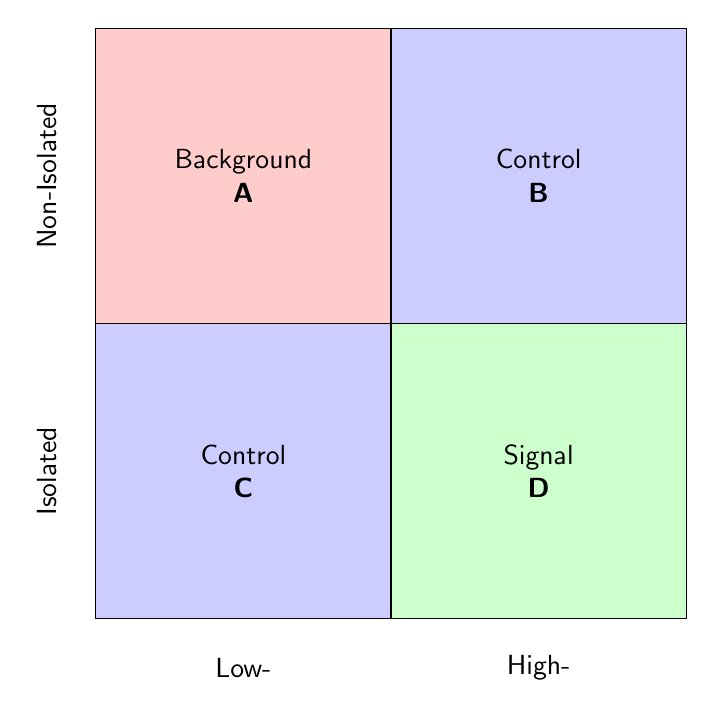
\begin{tikzpicture}[font=\sffamily]
  \tikzstyle{region}=[draw=black,minimum height=3.75cm,minimum width=3.75cm, fill=yellow!20,node distance=3.75cm,align=center]
  \tikzstyle{Signal}=[region, fill=green!20]
  \tikzstyle{Bkg}=[region,fill=red!20]
  \tikzstyle{Control}=[region,fill=blue!20]
  \tikzstyle{xLabel} = [font={\sffamily}, minimum width=3.75cm, node distance=3.75cm,node distance=2.5cm]
  \node[name=bkgregion, Bkg]{Background \\ \textbf{A}};
  \node[name=notIsolated, left of = bkgregion, xLabel, rotate=90] {Non-Isolated};
  \node[name=control1, right of = bkgregion, Control] {Control \\ \textbf{B}};
  \node[name=control2, below of = bkgregion, Control] {Control \\ \textbf{C}};
  \node[name=Isolated, left of = control2, xLabel, rotate=90] {Isolated};
  \node[name=signal, right of = control2, Signal] {Signal \\ \textbf{D}};
  \node[name=highMetLabel, xLabel, below of = signal] {High-\met};
  \node[name=lowMetLabel, xLabel, below of = control2] {Low-\met};
  \end{tikzpicture}  
  \caption{Diagram of the \met-isolation phase space. Shown are the four regions as defined by the event selection.}\label{fig:CrossSectionABCDRegions}
\end{figure}

These four regions are labelled A through D\@: A) a background-dominated region, containing events with low-\met\ and no isolated electrons; B) a control region with an isolated electron; C) a control region with low-\met; and D) the signal region, with events that pass the event selection. Events in each region represent a different multijet process that allows these to pass the event selection.

The tagging-rate is simply defined as
%
\begin{equation}
  R_{\textrm{SMT}}^{\textrm{multijet}} = \frac{N^{\textrm{multijet}}_{\textrm{tagged}}}{N^{\textrm{multijet}}_{\textrm{pretag}}} 
\end{equation}
%
where $N$ is the number of events in the region. Contaminations from non-multijet events such as $W$+jets, $Z$+jets, \ttbar, single-top, and diboson events are subtracted using MC simulation. Thus the yield in each region is defined as
%
\begin{equation}
  N^{\textrm{multijet}} = N^{\textrm{data}} - N^{W\textrm{+jets}} - N^{Z\textrm{+jets}} - N^{\ttbar} - N^{\textrm{diboson}} - N^{\textrm{single-top}}
\end{equation}

The largest sources of contamination are \ttbar, \W+jets, and \Z+jets, as shown in Table~\ref{tab:CrossContRegion} for pretag level and in Table~\ref{tab:CrossContRegionTagged} for tag level. Single-top and diboson contribute less than \SI{1}{\percent} in most bins and are therefore not shown here. As expected, Region A contains the least amount of contamination from other processes and is dominated by multijet events. Regions B and C are dominated by \W+jets in all jet-bins because of the presence a real lepton and \met\ from a real neutrino. The \Z+jets contamination is most significant in region C due to the requirement of an isolated electron but low-\met. 

\begin{table}[htbp]
  \centering
    \begin{tabular}{@{}S[input-comparators] % Jet bin Label
                  *{3}{S[table-format=2.2(2)]} % Contaminations
                    @{}}
      \toprule
      {Jet-bin} & \multicolumn{3}{c}{Contamination by [\si{\percent}]} \\
      \cmidrule{2-4}
              & {\ttbar} & {\W+jets} & {\Z+jets} \\
      \midrule
      \textbf{Region A} \\
      1       & 0.01(0)  & 6.99(2)   & 2.57(1)   \\
      2       & 0.13(1)  & 6.44(5)   & 3.87(4)   \\
      3       & 1.14(4)  & 5.72(10)  & 4.77(9)   \\
      $\geq$3 & 2.24(5)  & 5.64(9)   & 4.90(8)   \\
      \textbf{Region B} \\
      1       & 0.12(1)  & 39.1(1)   & 1.64(2)   \\
      2       & 1.47(3)  & 30.6(2)   & 2.61(5)   \\
      3       & 8.42(15) & 22.7(3)   & 3.21(9)   \\
      $\geq$3 & 14.0(2)  & 20.2(2)   & 3.14(8)   \\
      \textbf{Region C} \\
      1       & 0.02(0)  & 43.3(1)   & 20.0(4)   \\
      2       & 0.49(1)  & 36.4(1)   & 26.4(11)  \\
      3       & 4.63(9)  & 29.6(3)   & 29.9(3)   \\
      $\geq$3 & 8.77(11) & 28.0(2)   & 29.2(2)   \\
      \bottomrule
    \end{tabular}
    \caption[The portion of contamination in data in all control regions at pretag level.]{The portion of contamination in data in all control regions at pretag level. The uncertainties shown include statistical and systematic contributions.}\label{tab:CrossContRegion}
\end{table}

\begin{table}[htbp]
  \centering
    \begin{tabular}{@{}S[input-comparators] % Jet bin Label
                    *{3}{S[table-format=2.2(2)]} % Contaminations
                    @{}}
      \toprule
      {Jet-bin} & \multicolumn{3}{c}{Contamination by [\si{\percent}]} \\
      \cmidrule{2-4}
              & {\ttbar} & {\W+jets} & {\Z+jets} \\
      \midrule
      \textbf{Region A}                          \\
      1       & 0.05(2)   & 4.46(18) & 0.43(5)   \\
      2       & 0.82(12)  & 4.89(30) & 1.33(15)  \\
      3       & 5.64(54)  & 4.97(50) & 1.54(27)  \\
      $\geq$3 & 10.42(61) & 4.50(39) & 1.75(24)  \\
      \textbf{Region B}                          \\
      1       & 1.09(17)  & 26.6(9)  & 0.43(11)  \\
      2       & 8.71(55)  & 29.9(9)  & 1.02(18)  \\
      3       & 28.3(14)  & 12.2(8)  & 1.08(24)  \\
      $\geq$3 & 38.9(12)  & 9.84(53) & 0.95(16)  \\
      \textbf{Region C}                          \\
      1       & 0.36(7)   & 53.6(11) & 4.78(26)  \\
      2       & 4.86(36)  & 41.5(12) & 11.5(6)   \\
      3       & 26.5(14)  & 30.6(15) & 11.7(9)   \\
      $\geq$3 & 40.5(13)  & 24.2(10) & 10.1(6)   \\
      \bottomrule
    \end{tabular}
    \caption[The portion of contamination in data in all control regions at tagged level.]{The portion of contamination in data in all control regions at tagged level. The uncertainties shown include statistical and systematic contributions.}\label{tab:CrossContRegionTagged}
\end{table}

The distributions of various kinematic variables are shown in Figure~\ref{fig:CrossRegionB} after contamination is removed in region B. The \met\ distribution exhibits a long tail due to the aforementioned sources of fake reconstructed missing energy. The momentum distributions at both pretag and tag level point to the presence of  hard objects reconstructed as leptons in the multijet background likely coming from misidentified jets. The \xsd\ distribution of the SMT muons peaks at low \xsd\ values pointing to a good quality of fit between the ID and MS tracks of the muon. As expected the SMT muons are soft just as those in \ttbar\ events. One possible source of these soft muons is semileptonic decays of HF quarks.

% Multijet shapes region B
\begin{figure}[htbp]
  \centering
    \begin{subfigure}[b]{0.45\textwidth}
      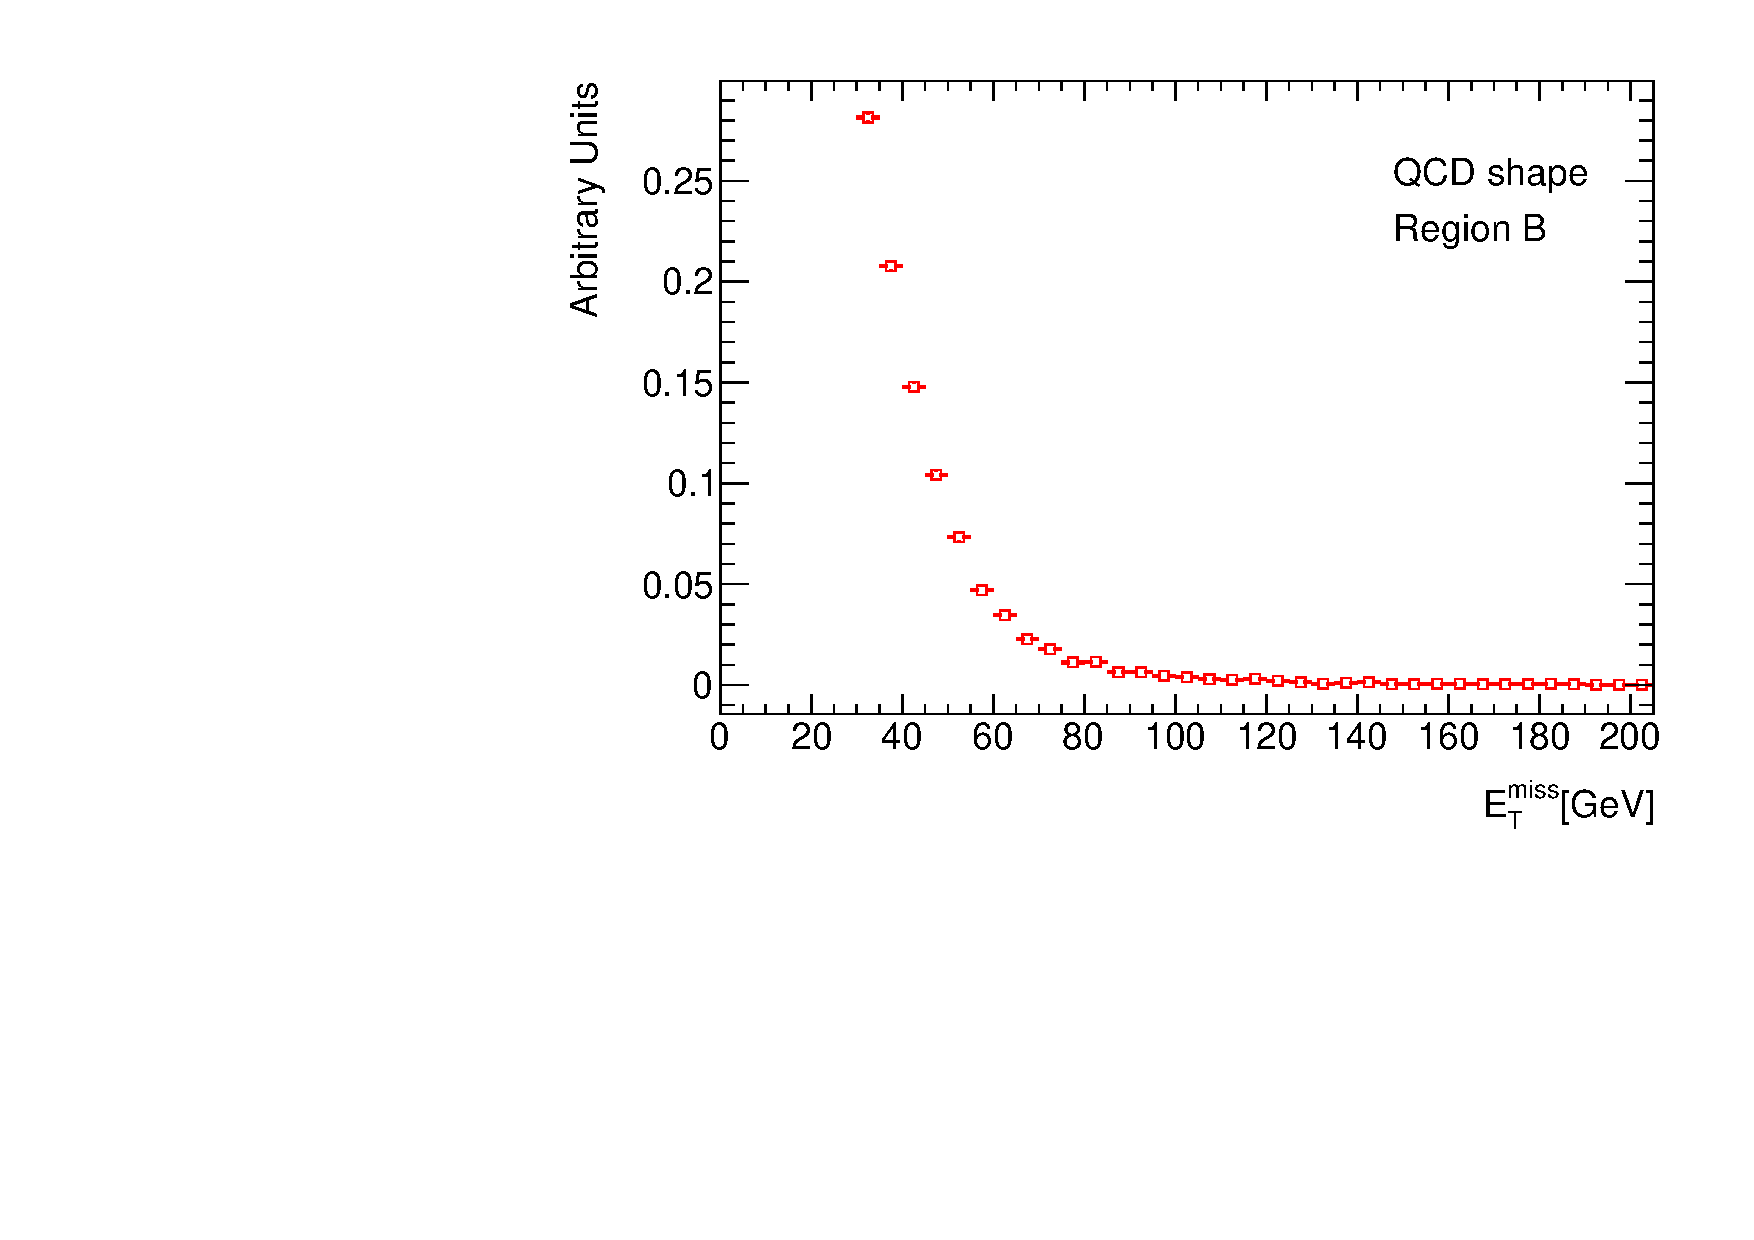
\includegraphics[width=0.95\textwidth]{PartCrossSection/Plots/Electron/h_el_pretag_MET_wgt.pdf}
      \caption{\met\ at pretag level}\label{fig:CrossRegionBpreMET}
    \end{subfigure}
    \;
    \begin{subfigure}[b]{0.45\textwidth}
      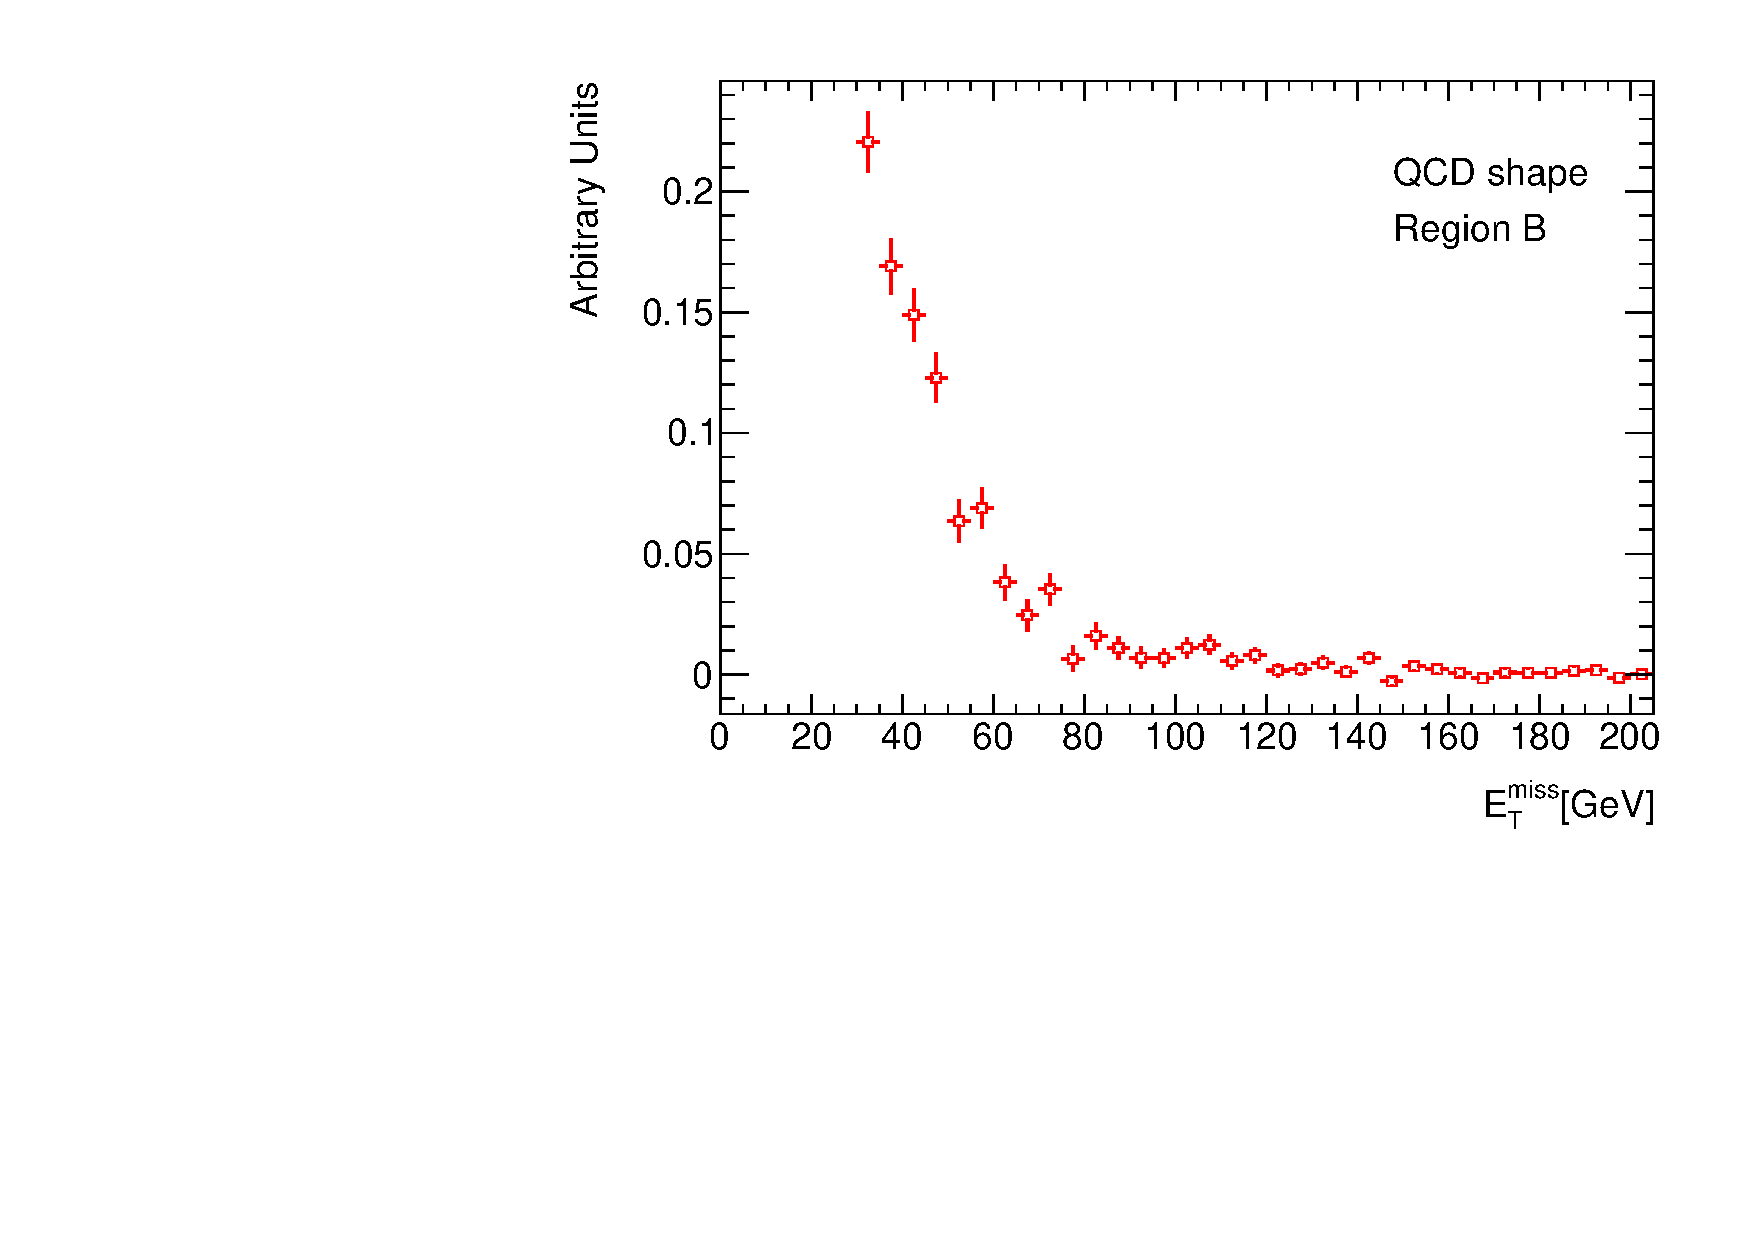
\includegraphics[width=0.95\textwidth]{PartCrossSection/Plots/Electron/h_el_tag_MET_wgt.pdf}
      \caption{\met\ at tag level}\label{fig:CrossRegionBTagMET}
    \end{subfigure}

    \begin{subfigure}[b]{0.45\textwidth}
      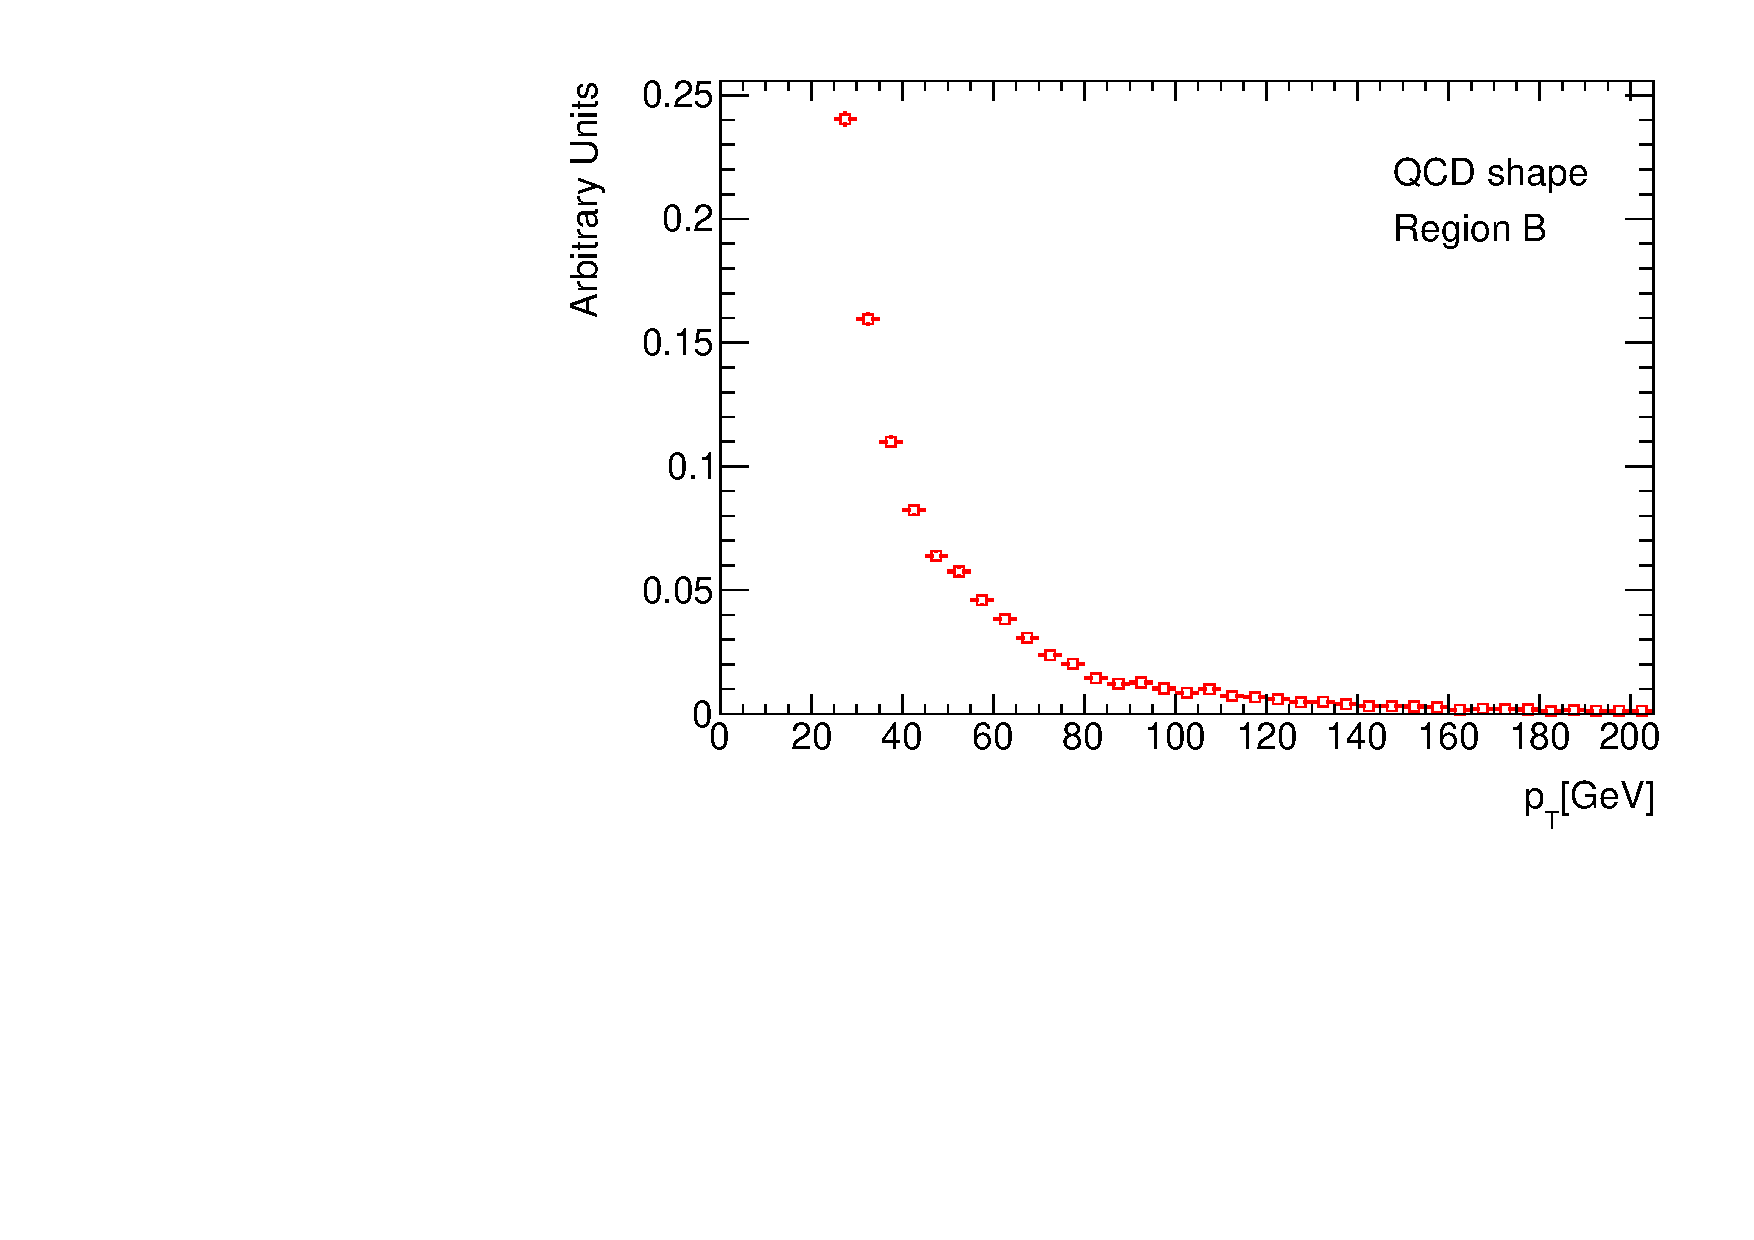
\includegraphics[width=0.95\textwidth]{PartCrossSection/Plots/Electron/h_el_pretag_pt_wgt.pdf}
      \caption{Electron \pt\ at pretag level}\label{fig:CrossRegionBPrePt}
    \end{subfigure}
    \;
    \begin{subfigure}[b]{0.45\textwidth}
      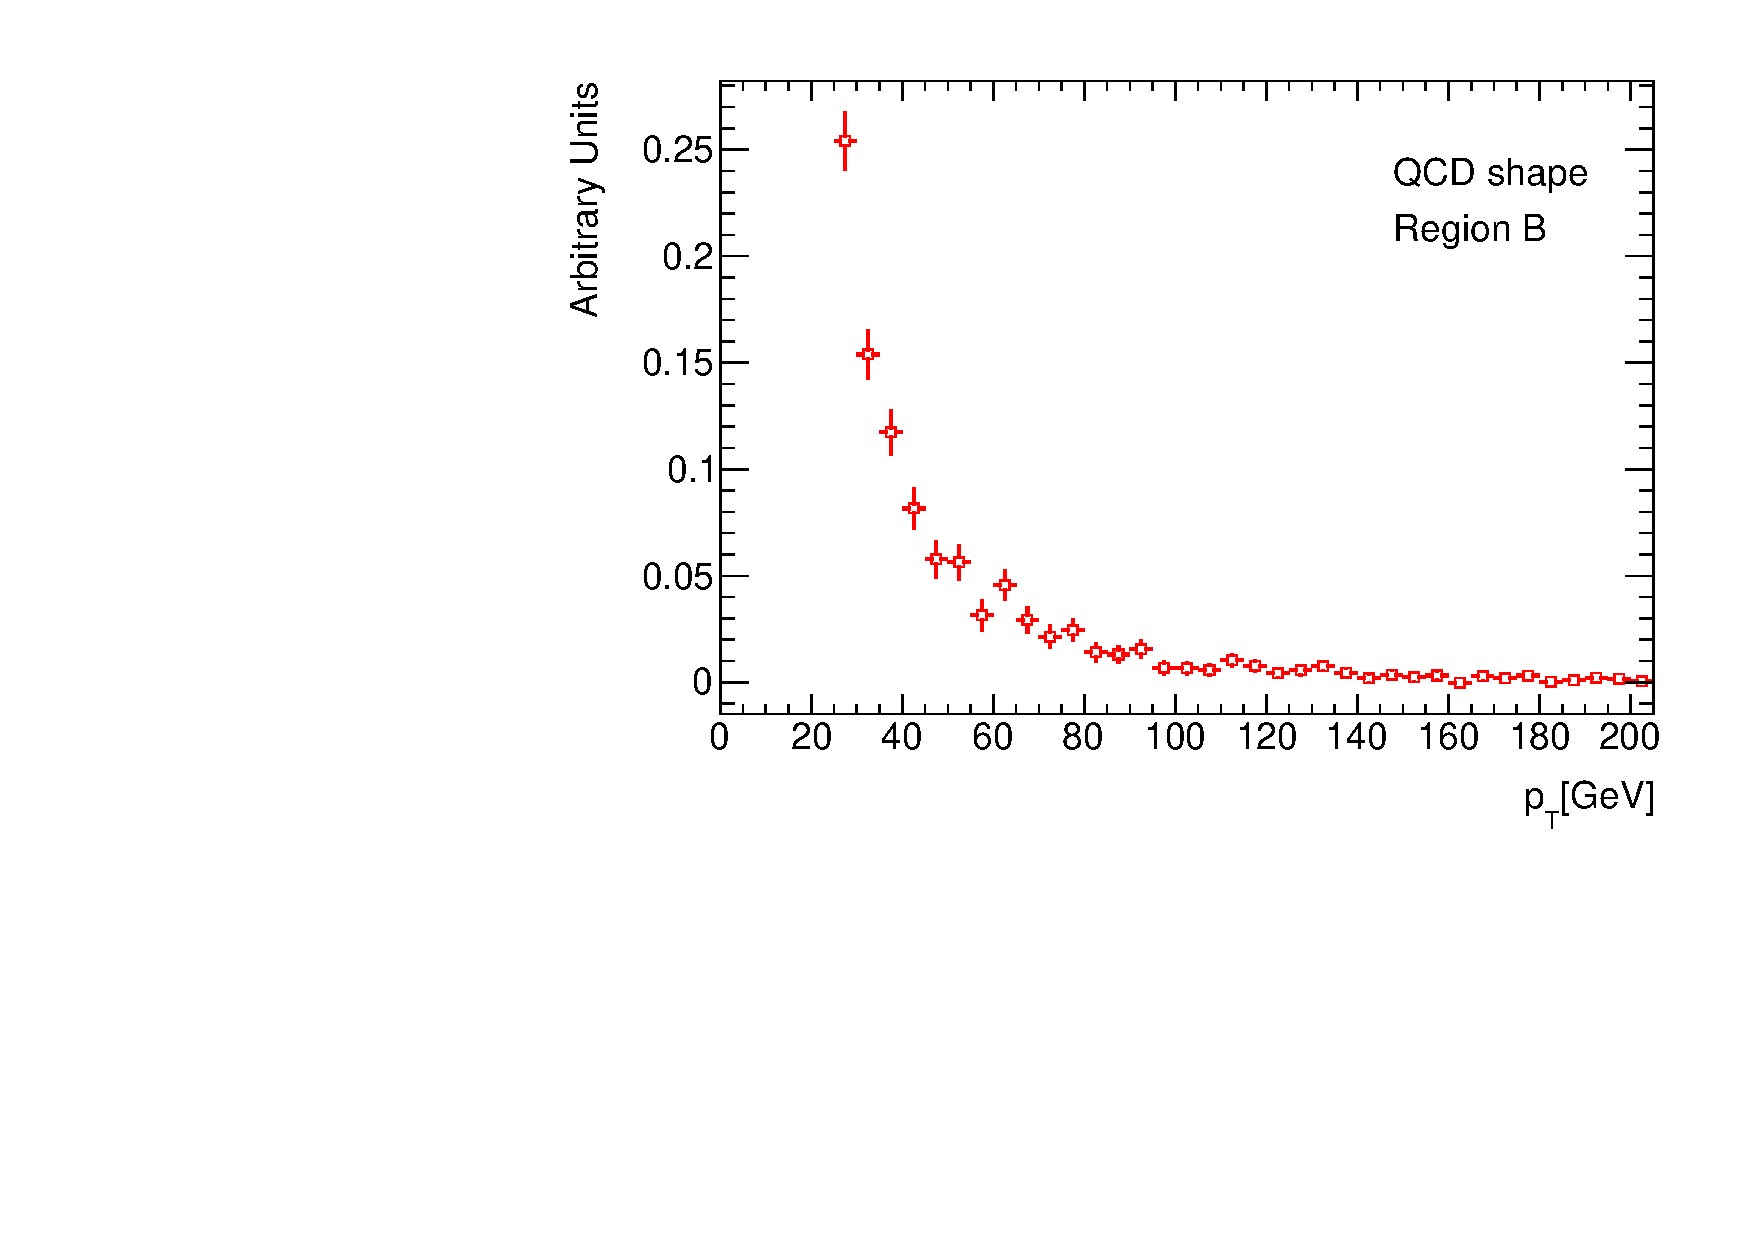
\includegraphics[width=0.95\textwidth]{PartCrossSection/Plots/Electron/h_el_tag_pt_wgt.pdf}
      \caption{Electron \pt\ at tag level}\label{fig:CrossRegionBTagPt}
    \end{subfigure}

    \begin{subfigure}[b]{0.45\textwidth}
      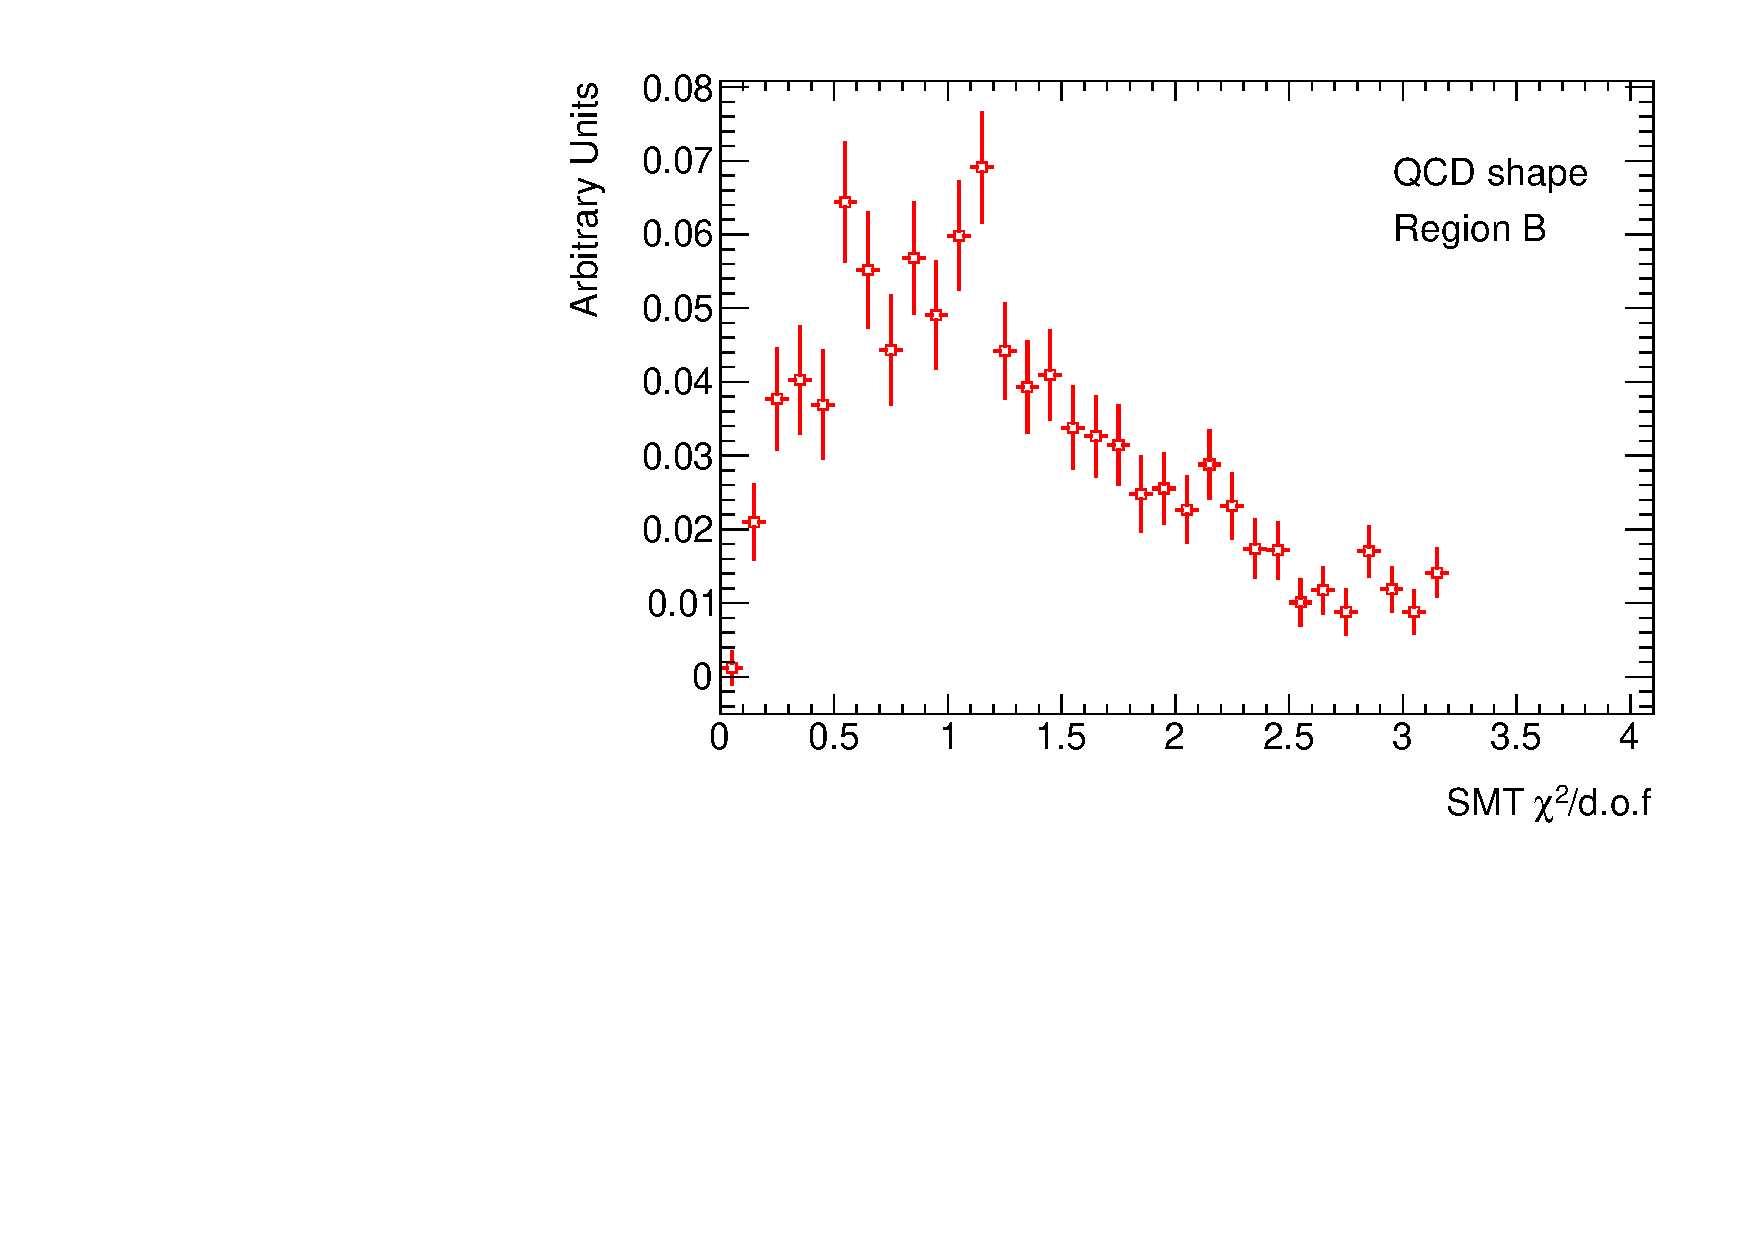
\includegraphics[width=0.95\textwidth]{PartCrossSection/Plots/Electron/h_el_tag_SMT_chi2_wgt.pdf}
      \caption{SMT muon \xsd\ at tag level}\label{fig:CrossRegionBChi2}
    \end{subfigure}
    \;
    \begin{subfigure}[b]{0.45\textwidth}
      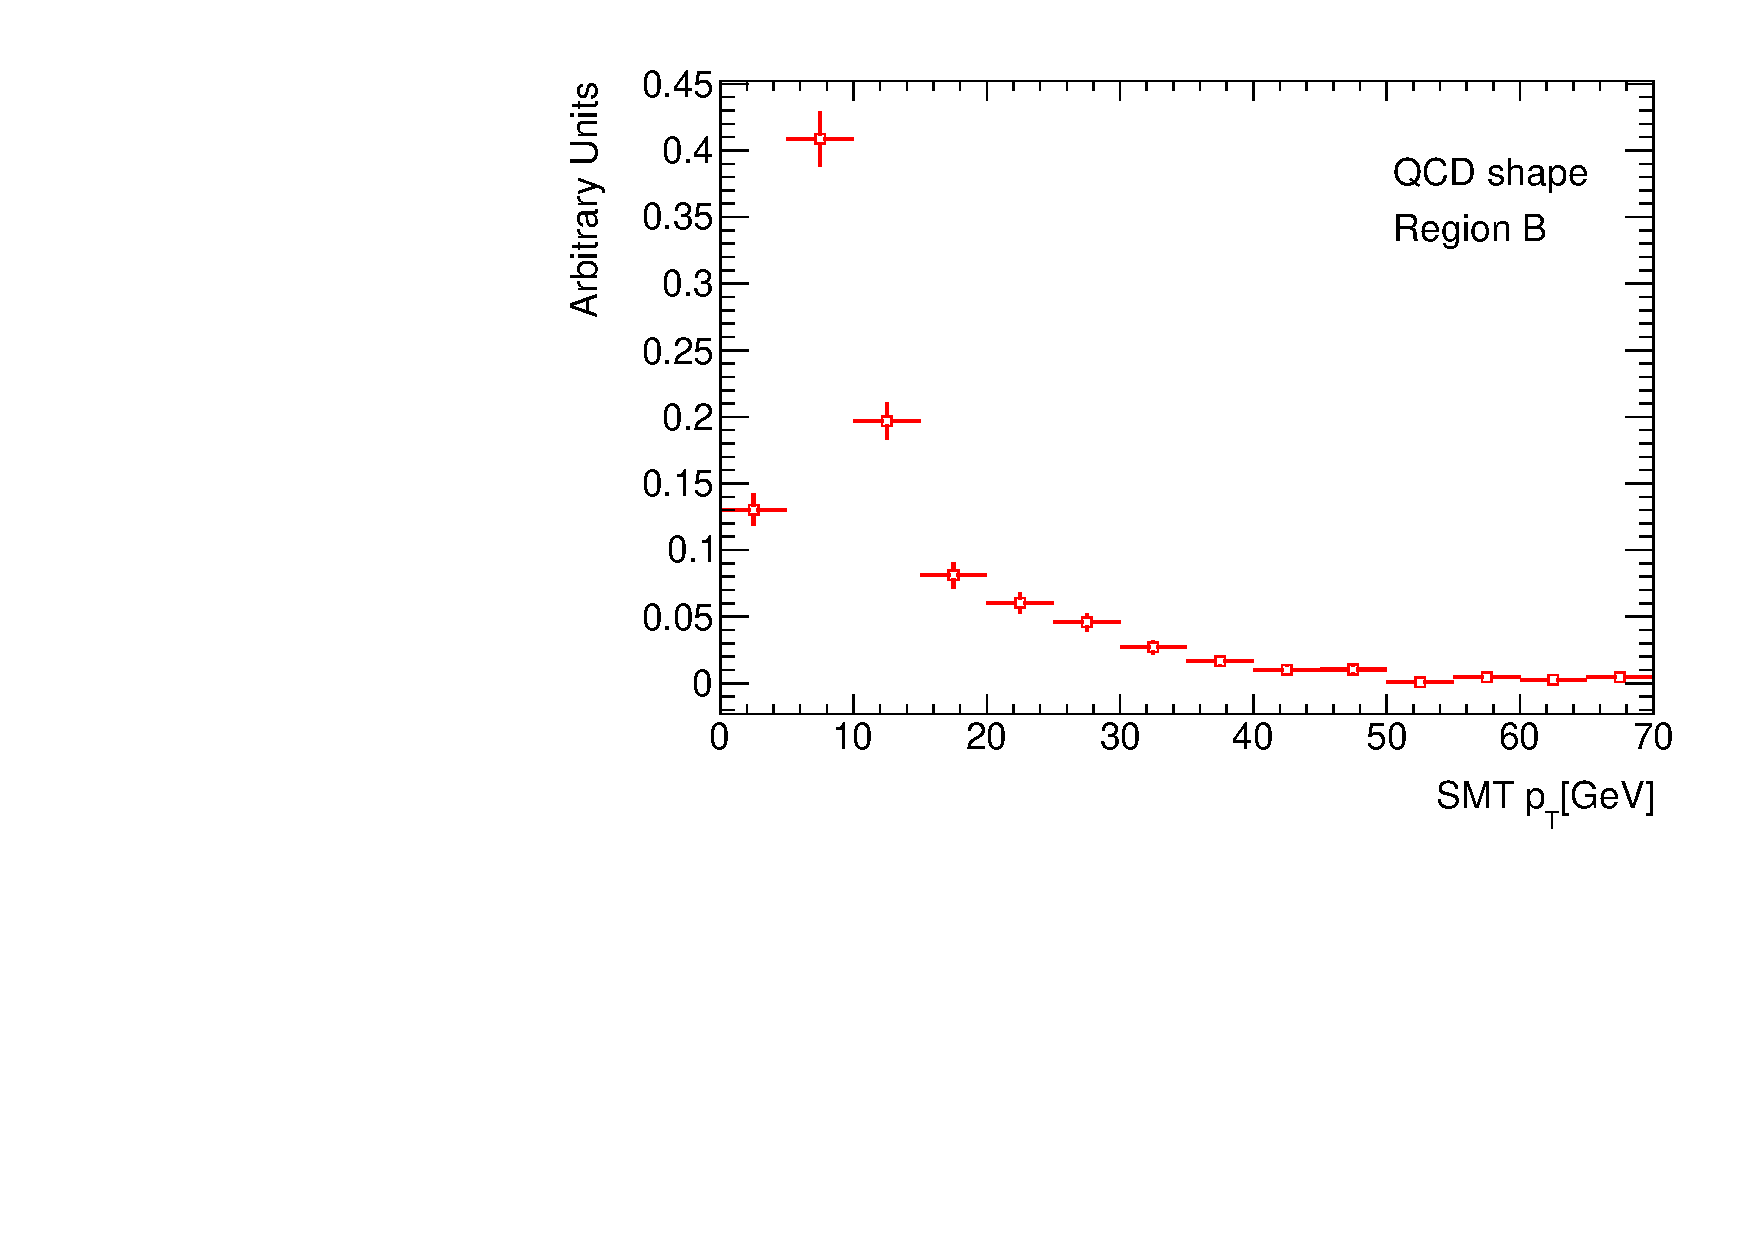
\includegraphics[width=0.95\textwidth]{PartCrossSection/Plots/Electron/h_el_tag_SMT_pt_wgt.pdf}
      \caption{SMT muon \pt\ at tag level}\label{fig:CrossRegionBSMTPt}
    \end{subfigure}
    \caption[Kinematic distributions measured in region B (high-\met\ and non-isolated) at pretag and tagged level.]{Kinematic distributions measured in region B (high-\met\ and non-isolated) at pretag and tagged level. These distributions are obtained by subtracting non-multijet contributions using simulation.}\label{fig:CrossRegionB}
\end{figure}

The normalization of the \ttbar\ contribution is initially based on the theoretical cross section. An estimate for the multijet contribution is determined using this cross section and a new measured \ttbar\ cross section is obtained. This cross section is used to rescale the \ttbar\ contribution and a new cross section is obtained. This process is repeated until the measured cross section stabilizes. Only two iterations are needed.

The uncertainty on the tagging-rate contains statistical and systematic contributions. The systematic uncertainty includes the uncertainty on the cross section of the \ttbar\ and $W$+jets samples, \SI{15}{\percent} and \SI{25}{\percent} respectively; uncertainty from the calibration of the SMT tagger; and uncertainties associated with the BR re-weighting. For more detail on the tagger-specific uncertainty, see Section~\ref{sec:systematics_uncertainties}. The dominant source of uncertainty depends on the region and jet-bin. In regions where contamination is high, the uncertainty from \W+jets and \ttbar\ are more significant.

The final tagging-rate is the unweighted average of all three regions. This definition was chosen as no single type of multijet process is favoured over the others. The uncertainty is half the largest difference in rates between the regions. This covers the entire range of possible tagging-rate values. The tagging-rates per region for each jet-bin, including uncertainty, are shown in Table~\ref{tab:rsmt}.

\begin{table}[htbp]
  \centering
    \begin{tabular}{@{}S[input-comparators] % Jet-bin label
                       S[table-format=0.2(1)] % 
                       S[table-format=1.2(1)] %
                       S[table-format=1.3(3)] %
                       S[table-format=1.3(3)] %
                    @{}}
        \toprule
        {Jet-bin} & \multicolumn{4}{c}{SMT tagging-rate $R^{\textrm{SMT}}$ [\si{\percent}]} \\
        \cmidrule{2-5}
                & {Region A} & {Region B} & {Region C} & {Average}   \\ 
        \midrule
        1       & 1.17(1)    & 1.10(10)   & 0.609(56)  & 0.962(446) \\
        2       & 2.25(3)    & 2.49(10)   & 1.55(17)   & 2.09(47)   \\
        3       & 3.44(9)    & 4.31(21)   & 2.27(85)   & 3.34(102)  \\
        $\ge$3  & 3.84(9)    & 5.14(41)   & 2.52(130)  & 3.83(131)  \\
        % 4       & 4.87(24)   & 5.71(91)   & 2.52(360)  & 4.37(279)  \\
        % $\ge$4  & 5.33(25)   & 7.17(95)   & 3.58(390)  & 5.36(271)  \\
        \bottomrule
    \end{tabular}
    \caption{Results of the SMT multijet tagging-rate measurement in region A) inverted-\met, non-isolated, B) High-\met, non-isolated and C) low-\met, isolated.}\label{tab:rsmt}
\end{table}

The multijet background estimates in the $e$+jets channel are shown in Table~\ref{tab:rsmtest}. The uncertainties on the final pretag and tagged estimates are dominated by the \SI{50}{\percent} uncertainty on the efficiencies associated with the matrix method pretag estimate.

\begin{table}[!htbp]
  \centering
    \begin{tabular}{@{}
                    S[input-comparators] % Label
                    S[table-format=6(5)] % Pretag
                    S[table-format=4(3)] % Tagged
                    @{}}
      \toprule
      {Jet-bin} & \multicolumn{2}{c}{Multijet event yield} \\
      \cmidrule{2-3}
                & {Pretag}      & {Tagged}        \\
      \midrule
      1         & 145000(72000) & 1390(700)       \\ 
      2         & 39600(19800)  & 830(416)        \\
      3         & 11300(5700)   & 378(190)        \\ 
      $\ge$3    & 16200(8100)   & 620(311)        \\
      % 4         & 3320(1660)    & 145(74)         \\
      % $\ge$4    & 4860(2430)    & 260(130)        \\
      \bottomrule
    \end{tabular}
    \caption[Results of the matrix method estimation of the multijet background in the $e$+jets channel.]{Results of the matrix method estimation of the multijet background in the $e$+jets channel. The uncertainties are combined statistical and systematics.}\label{tab:rsmtest}
\end{table}

\subsubsection{The ABCD method}
The ABCD method relies on a pair of uncorrelated variables to extrapolate the amount of multijet events from a set of control regions into the signal region. First, a two-dimensional phase-space is constructed, in this case the same construct shown in Figure~\ref{fig:CrossSectionABCDRegions} is used. If these two variables are uncorrelated then the following relation holds
%
\begin{align}
  \frac{N^{\textrm{multijet}}_{\textrm{D}}}{N^{\textrm{multijet}}_{\textrm{C}}} &= \frac{N^{\textrm{multijet}}_{\textrm{B}}}{N^{\textrm{multijet}}_\textrm{A}}
\end{align} 
%
where $N^{\textrm{Multijet}}_{\textrm{X}}$ is the number of multijet events in region X. As with the matrix method, the value of $N^{\textrm{Multijet}}$ is obtained by subtracting the contribution of other processes from the data value using simulation.

This allows an estimation of the number of multijet events that pass the event selection by extrapolating from the background region into the signal region. The uncertainty on the final estimate includes statistical contributions from the yield in each region and the systematic uncertainty on the $W$+jets and \ttbar\ samples as described. The multijet estimates in all regions at pretag and tagged level are presented in Table~\ref{tab:CrossABCDEstimates}. The uncertainty on the estimate in some jet-bins is smaller than the matrix method estimate. However, in the signal jet-bin ($\geq$3) the uncertainty at tag level is very large. The matrix method estimate is therefore used as the central value and the ABCD estimate is used as a cross-check. Comparing the results from the matrix method and the ABCD method, it appears that both produce compatible results within their uncertainties.

\begin{table}
  \centering
    \begin{tabular}{@{}
                    S[input-comparators] % Jet bin Label
                    S[table-format=5(5)]
                    S[table-format=3(3)]
                    @{}}
      \toprule
      {Jet-Bin} & \multicolumn{2}{c}{Multijet event yield} \\
      \cmidrule{2-3}
                & {Pretag}     & {Tag}                     \\
      \midrule
      1         & 99000(48000) & 565(264)                  \\
      2         & 33500(13000) & 572(272)                  \\
      3         & 9500(3320)   & 270(220)                  \\
      $\geq$3   & 13000(5000)  & 438(449)                  \\
      % 4         & 2350(1140)   & 69(135)                   \\
      % $\geq$4   & 3380(1700)   & 162(254)                  \\
      \bottomrule
      \end{tabular}
    \caption[Results of the ABCD method estimation of the multijet background in the $e$+jets channel.]{Results of the ABCD method estimation of the multijet background in the $e$+jets channel. The uncertainty contains statistical and systematic components.}\label{tab:CrossABCDEstimates}
\end{table}

\subsection{Multijet background in the muon channel}

The procedure in the muon channel is similar to that used for the electron channel. A pretag estimate of the multijet fraction in the signal region is obtained using the matrix method. The ``real'' muon selection efficiency $r$ is measured from an inclusive sample of $Z\rightarrow\mu\mu$ events. The ``fake'' muon selection efficiency $f$ is obtained from data using two different samples:

\begin{itemize}
  \item A background-dominated control region where the $\met+\mtw$ cut is inverted and an additional cut of $\mtw<\SI{20}{\GeV}$ is applied.
  \item A fit to the transverse impact parameter significance  distribution where both $\met+\mtw$ and \met\ cuts are inverted.
\end{itemize}

The central value of the pretag estimate is obtained from an average of these two regions and was found to be \num{27000(5400)}. An uncertainty of \SI{20}{\percent} is assigned to the final estimate to account for the uncertainty associated with each region and the difference between them. 

The SMT event tagging-rate is obtained from two control regions defined by inverting the \met\ and $\met+\mtw$ cuts, and by inverting the muon isolation requirement. As with the electron analysis, contamination from other non-multijet processes is subtracted using MC simulation. The associated sources of uncertainty are the same as those considered in the electron channel.

\begin{table}
  \centering
    \begin{tabular}{@{}lS[table-format=1.1(1)]@{}}
      \toprule
      Control region & {SMT tagging-rate [\si{\percent}]}  \\
      \midrule
      Inverted isolation      & 5.7(1) \\
      Inverted triangular cut & 4.0(5) \\
      \midrule
      Unweighted average      & 4.9(8) \\
      \bottomrule
    \end{tabular}
    \caption[Summary of tagging-rates as measured in data in the two multijet-dominated regions.]{Summary of tagging-rates as measured in data in the two multijet-dominated regions. The uncertainty quoted includes statistical and systematic contributions. The uncertainty on the unweighted average is set as half of the difference between control regions~\cite{Cross:SMTCrossSectionPaper}.}\label{tab:CrossMuonQCDTaggings}
\end{table}

The final multijet estimate at tagged level is obtained by multiplying the average pretag estimate by the unweighted tagging-rate. The uncertainty on the unweighted tagging-rate is set to half the difference between the two control regions, as this is larger than the individual uncertainties combined. The final uncertainty is obtained by combining the uncertainties on the pretag estimate and the tagging-rate. The final tagged estimate was found to be \num{1310(350)}.

\subsection{\emph{W}+jets background}

The \W+jets background is the most dominant background since these events contain a real lepton and \met\ from the escaping neutrino. Events can be classified into \W+HF, which is the largest contribution; and \W+LF where a LF jet is mistagged. Due to the significant uncertainty on the overall normalization of \W+jets and the presence of a mistagged LF jet, a data-driven method known as \W\ charge asymmetry~\cite{Measurement} is used to estimate this background.

The \W\ charge asymmetry method relies on the charge asymmetry in the production of \W-bosons. As the LHC is a proton-proton collider, up-type valence quarks are more prevalent, resulting in an increased rate of \Wplus\ production via $u\bar{d}\rightarrow\Wplus$ or $c\bar{s}\rightarrow\Wplus$ compared to \Wminus\ production involving down-type quarks. The ratio of these production cross sections $r$ is theoretically well understood~\cite{Cross:WChargeAsymmetry}. It is thus possible to use this ratio as measured in MC simulation to determine an overall normalization in data from the following formula: 
%
\begin{align}
  N_{W^{+}}+N_{W^{-}} &= \frac{N^{\textrm{MC}}_{W^{+}} + N^{\textrm{MC}}_{W^{-}} }{ N^{\textrm{MC}}_{W^{+}} - N^{\textrm{MC}}_{W^{-}} } (D^{+} - D^{-}) \\
                      &= \frac{r_{\textrm{MC}} + 1}{r_{\textrm{MC}} - 1} (D^{+} - D^{-})
\end{align}
%
where $r_{\textrm{MC}}$ is the ratio as measured in MC and $D^{\pm}$ are the number of events in data with a positively- or negatively-charged lepton. Contributions from other charge asymmetric processes, namely single-top and diboson are removed using MC simulation. This results in an overall normalization for the \W+jets background at the pretag level. The flavour of the quarks produced in association with the \W-boson is particularly important when performing $b$-tagging. Events are categorized by the flavour of these accompanying quarks into $Wc$+jets, $Wb\bar{b}$+jets, $Wc\bar{c}$+jets and \W+LF\@. The tagged level estimate is obtained by multiplying the pretag estimate via a tagging-rate, obtained separately for $b\bar{b}$, $c\bar{c}$, $c$ and LF separately. The overall tagged estimate is then obtained using the following formula:
%
\begin{equation}
  W_{\textrm{tag}} = R^{\textrm{LF}}_{\textrm{tag}}W^{\textrm{LF}}_{\textrm{pretag}} + \sum_{\textrm{HF}}^{\textrm{HF}=c,cc,bb} R^{\textrm{HF}}_{\textrm{tag}}W^{\textrm{HF}}_{\textrm{pretag}}
\end{equation}
% 
where $R^{\textrm{LF}}_{\textrm{tag}}$ is defined as the probability to mistag a LF event and $R^{\textrm{HF}}_{\textrm{tag}}$ is the probability to correctly tag a HF event. The tagging-rates are obtained from simulation with the SMT scale factors and BR reweighing applied to each tagged jet. The results of the estimation are summarized in Table~\ref{tab:CrossWJetsSummary}.

\begin{table}
  \centering
    \begin{tabular}{@{}lS[table-format=6(4)]S[table-format=4(3)]@{}}
      \toprule
      Channel  & \multicolumn{2}{c}{$W$+jets event yield} \\
               & {Pretag}     & {Tagged}  \\
      \midrule
      \ejets\  & 59300(5400)  & 1640(330) \\
      \mujets\ & 117200(9300) & 2900(500) \\
      \bottomrule
    \end{tabular}
    \caption[Results of the $W$+jets background estimation at pretag and tagged level for the three-jets inclusive selection.]{Results of the $W$+jets background estimation at pretag and tagged level for the three-jets inclusive selection~\cite{Cross:SMTCrossSectionPaper}.}\label{tab:CrossWJetsSummary}
\end{table}

\subsection{Background shapes}

Kinematic distributions are shown at the tagged level in Figures~\ref{fig:CrossBackgroundShapes} for events with at least three jets in both electron and muon channels. The multijet distributions are taken from data normalized to the obtained estimates. In the electron channel, the multijet shapes are obtained from region B, as defined in Figure~\ref{fig:CrossSectionABCDRegions}, with the contamination from non-multijet processes removed. The multijet shapes in the muon channel are obtained from the loose selection in data, after the application of per-event weights obtained from the matrix method.
SMT muon distributions for both background and signal are shown in Figure~\ref{fig:CrossBackgroundSMTShapes}. It is noted that the \xsd\ distribution is shifted in both channels in data compared to the simulation. Any such discrepancies are accounted for by the \xsd\ scale factor. Good agreement between data and estimations, both simulation-based and data-driven, is observed in all distributions.

\begin{figure}[htbp]
  \centering
    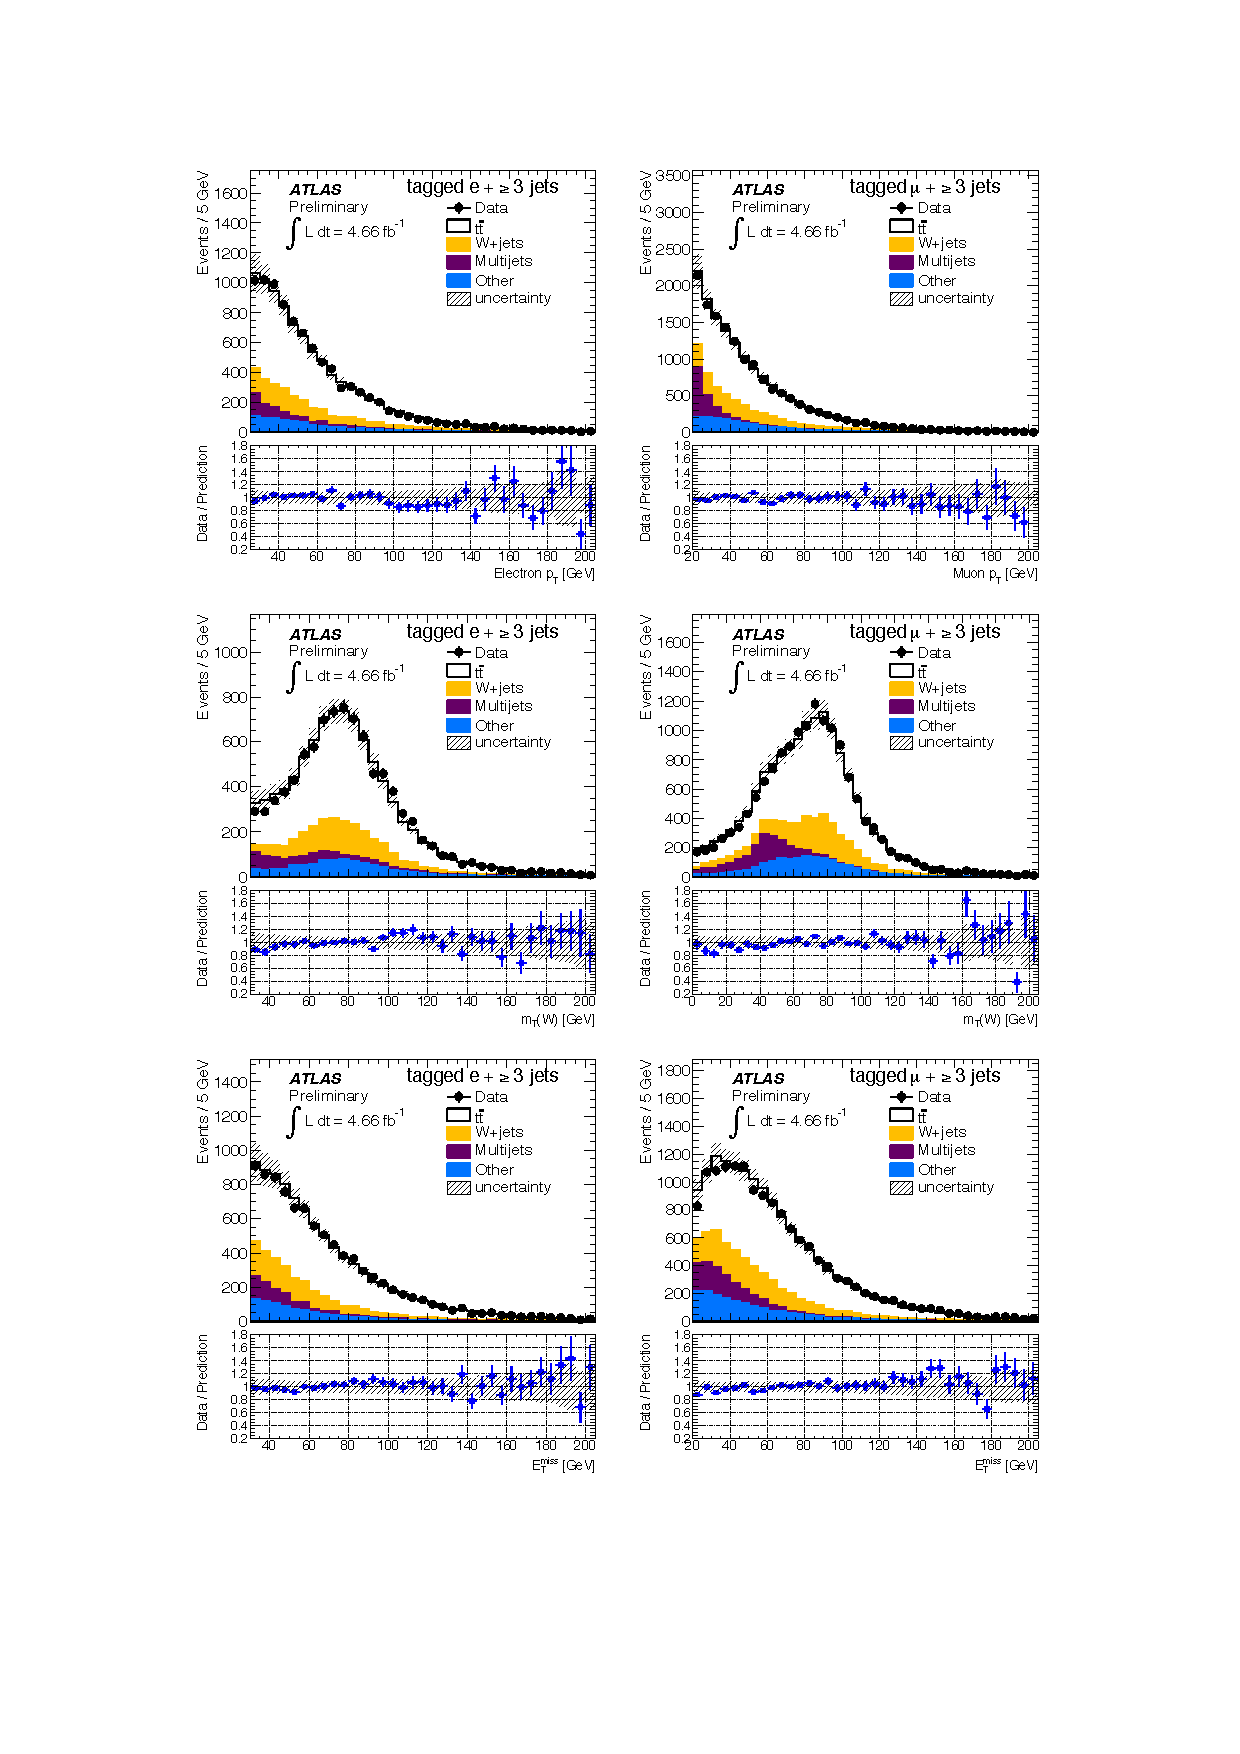
\includegraphics[width=0.90\textwidth]{PartCrossSection/Plots/h_stacks_elmu_evt_pars.pdf}
    \caption[Distributions for tagged events in the \ejets\ (left) and \mujets\ (right) channels of (from top to bottom): lepton \pt, transverse $W$ mass, and missing transverse energy.]{Distributions for tagged events in the \ejets\ (left) and \mujets\ (right) channels of (from top to bottom): lepton \pt, transverse $W$ mass, and missing transverse energy~\cite{Cross:SMTCrossSectionPaper}.}\label{fig:CrossBackgroundShapes}
\end{figure}

\begin{figure}[htbp]
  \centering
    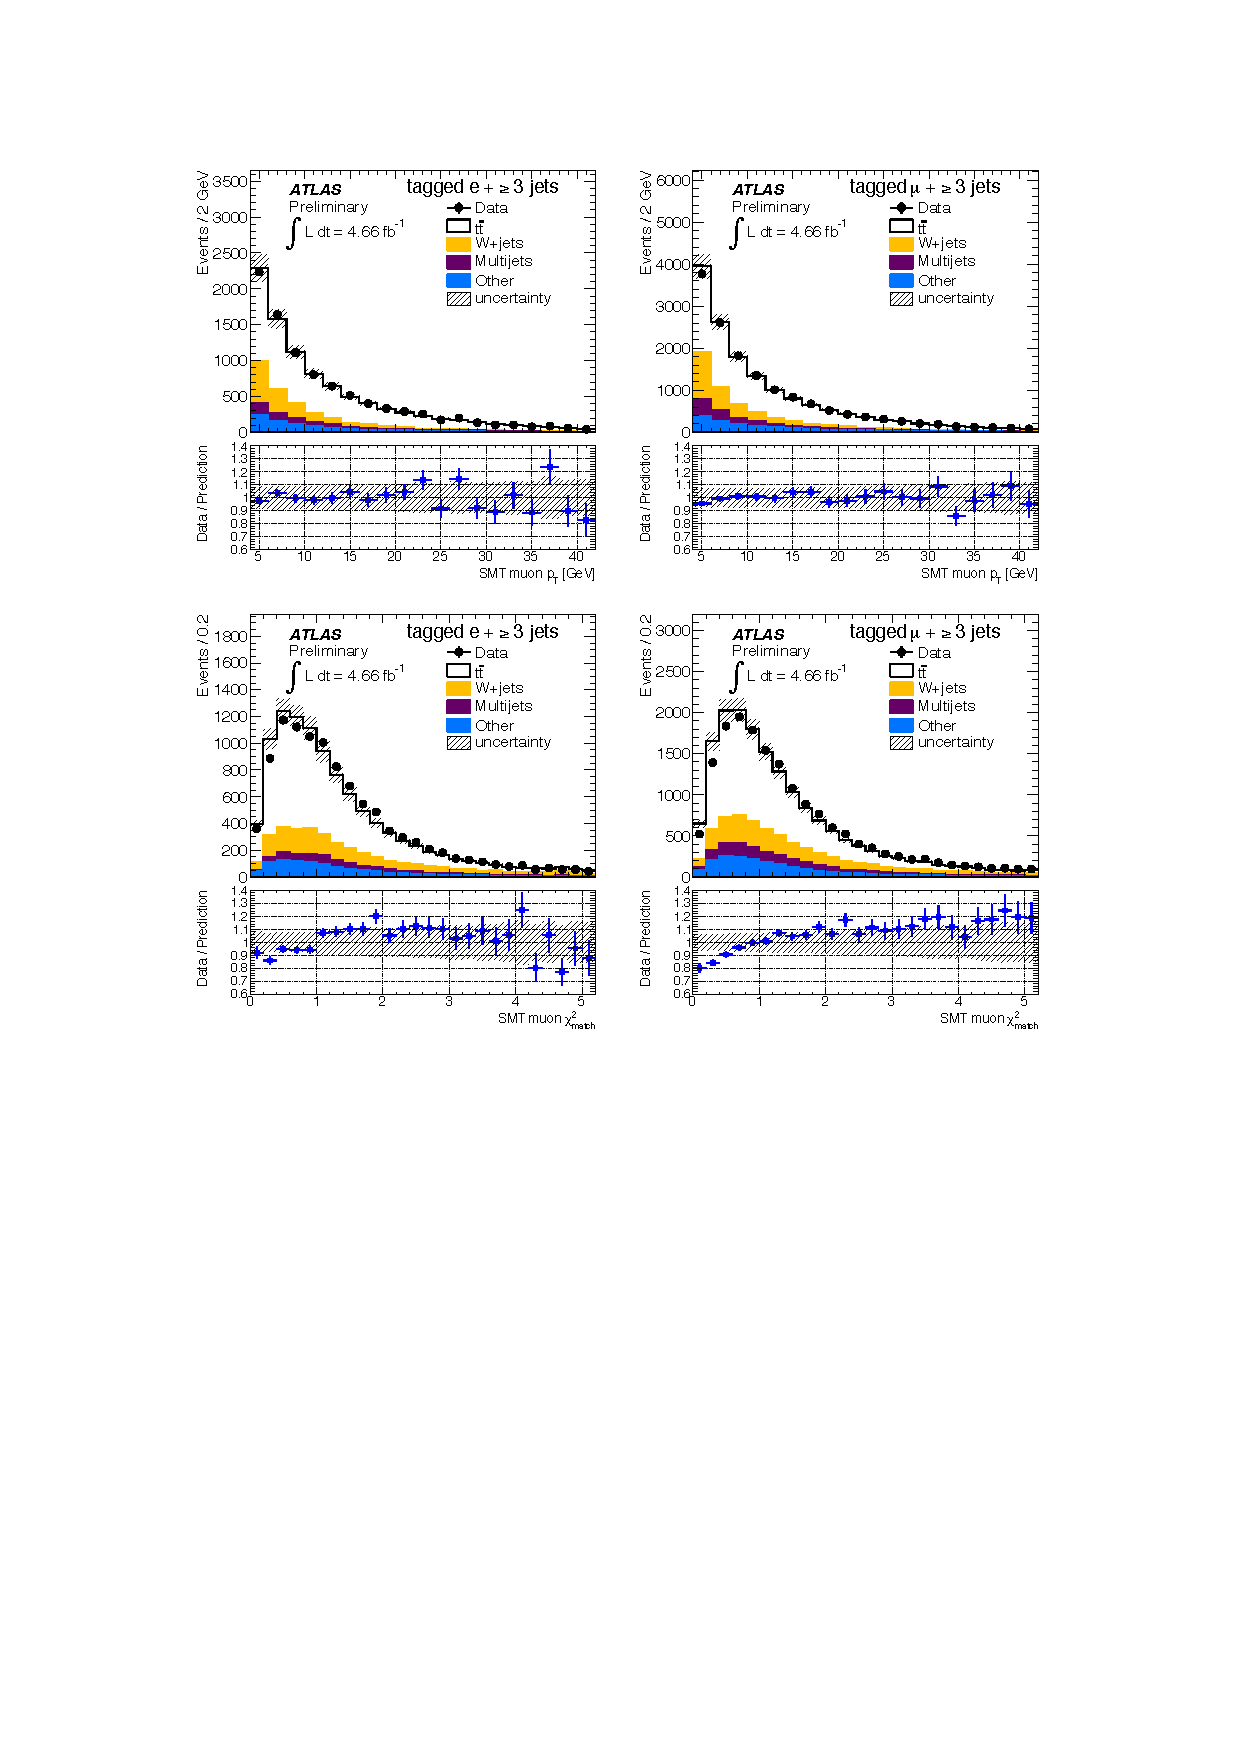
\includegraphics[width=0.90\textwidth]{PartCrossSection/Plots/h_stacks_elmu_SMT_pars.pdf}
    \caption[Distributions of SMT variables in the \ejets\ (left) and \mujets\ (right) of (from top to bottom): SMT muon \pt\ and SMT muon \xsd.]{Distributions of SMT variables in the \ejets\ (left) and \mujets\ (right) of (from top to bottom): SMT muon \pt\ and SMT muon \xsd~\cite{Cross:SMTCrossSectionPaper}.}\label{fig:CrossBackgroundSMTShapes}
\end{figure}


\section{Systematic uncertainties}\label{sec:systematics_uncertainties}

The uncertainties associated with the cross section include various sources such as signal simulation, object reconstruction, background estimation, integrated luminosity determination and tagger uncertainties (Table~\ref{tab:CrossSectionUncertainty}). The SMT tagger uncertainty is made of the STACO CB reconstruction uncertainty and the uncertainty on the \xsm\ efficiency measurement. 

The signal modelling uncertainties are evaluated by repeating the cross section measurement while substituting the main \ttbar\ sample with alternate ones. The NLO generator uncertainty covers any differences in the modelling of kinematic distributions at parton level as a result of the hard interaction in different generators. This is evaluated by comparing the signal acceptance in ALPGEN and POWHEG~\cite{Cross:PowHegGeneral,Cross:PowHegBox} samples to the nominal sample. Initial and final state radiation (ISR/FSR) uncertainty covers the differences in modelling of soft radiation from initial and final state particles. This uncertainty is evaluated in studies on samples generated with AcerMC and PYTHIA, and by varying parameters which affect ISR/FSR simulation in the range consistent with experimental data~\cite{Cross:ISRFSROne,Cross:ISRFSRTwo}. The PDF uncertainty is evaluated using three PDF sets: the nominal CT10~\cite{Cross:CT10}, MSTW~\cite{Cross:MSTW2008}, and NNPDF~\cite{Cross:NNPDF}. Several uncertainties are related to each PDF set. Each variation is evaluated by an event-by-event re-weighting of the signal \ttbar\ MC. The total uncertainty assigned to $\sigma_{\ttbar}$ is then half the spread of the envelope of all PDF uncertainties~\cite{Cross:SMTCrossSectionPaper}.

The largest uncertainties come from the background estimation methods, JES corrections, and SMT tagger uncertainties. In the multijet background estimate, the uncertainty associated with the matrix method pretag estimates is the largest contribution at \SI{50}{\percent} of the estimate. The tagger uncertainties, including the $b\rightarrow\mu X$ BR re-weighting uncertainty, contribute approximately $+\SI{3.2}{\percent}/-\SI{3.4}{\percent}$ to the total uncertainty. In comparison, the total $b$-tagging uncertainty as measured by another $\ell$+jets analysis using JetProb is $+\SI{4.1}{\percent}/-\SI{3.8}{\percent}$~\cite{Cross:BtaggingExample}. This is larger than the total SMT tagger uncertainty despite including the BR re-weighting uncertainty. Overall, the analysis is dominated by the systematic uncertainty and reduced acceptance due to the BR of $b\rightarrow \mu$ is not significant in this case.

\begin{table}[htpb]
  \centering
  \begin{tabular}{@{}l*{3}{c}@{}}
    \toprule
    Source & \multicolumn{3}{c}{Relative cross section uncertainty [\si{\percent}]} \\
            \cmidrule{2-4}
           & {\ejets} & {\mujets} & Combined \\
    \midrule
    \textbf{Statistical Uncertainty}     & $\pm1.5$          & $\pm1.3$       & $\pm1.0$       \\
    \textbf{Object Selection}                                                                  \\
    \tabin\ Lepton Energy Resolution      & $+0.4/-0.3$       & $+0.2/-0.01$   & $+0.2/-0.1$    \\
    \tabin\ Lepton Reco., ID, Trigger     & $+2.4/-2.5$       & $+1.5/-1.5$    & $+1.5/-1.8$    \\
    \tabin\ Jet Energy Scale              & $+3.8/-4.3$       & $+3.2/-3.6$    & $+3.5/-3.8$    \\
    \tabin\ Jet Energy Resolution         & $\pm0.2$          & $\pm0.5$       & $\pm0.2$       \\
    \tabin\ Jet Reconstruction Efficiency & $\pm0.06$         & $\pm0.06$      & $\pm0.06$      \\
    \tabin\ Jet Vertex Fraction           & $+1.2/-1.4$       & $+1.2/-1.4$    & $+1.2/-1.4$    \\
    \tabin\ \met\ Uncertainty             & $\pm0.06$         & $\pm0.08$      & $\pm0.07$      \\
    \textbf{SMT Calibration}                                                                   \\
    \tabin\ STACO Reconstruction Eff.     & $\pm\num{1.3}$    & $\pm\num{1.3}$ & $\pm\num{1.3}$ \\ 
    \tabin\ Muon \xsm\ Eff.               & $\pm\num{0.6}$    & $\pm\num{0.6}$ & $\pm\num{0.6}$ \\
    \textbf{Background Estimates}                                                              \\
    \tabin\ Multijet Normalisation        & $\pm\num{5.2}$    & $\pm\num{3.9}$ & $\pm\num{4.4}$ \\
    \tabin\ $W$+jets Normalisation        & $\pm\num{5.2}$    & $\pm\num{5.7}$ & $\pm\num{5.5}$ \\
    \tabin\ Other Bkg Normalisation       & $\pm\num{0.2}$    & $\pm\num{0.2}$ & $\pm\num{0.1}$ \\
    \tabin\ Other Bkg Systematics         & $+1.6/-1.5$       & $+2.5/-2.0$    & $+2.2/-1.8$    \\
    \textbf{Signal Simulation}                                                                 \\
    \tabin\ $b\rightarrow \mu X$ %
            Branching Ratio              & $+2.9/-3.0$       & $+2.9/-3.1$    & $+2.9/-3.1$    \\
    \tabin\ ISR/FSR                       & $\pm\num{2.4}$    & $\pm\num{0.9}$ & $\pm\num{1.5}$ \\
    \tabin\ PDF                           & $\pm\num{3.2}$    & $\pm\num{3.0}$ & $\pm\num{3.1}$ \\
    \tabin\ NLO Generator                 & $\pm\num{3.2}$    & $\pm\num{3.2}$ & $\pm\num{3.2}$ \\
    \tabin\ Parton Shower                 & $\pm\num{2.2}$    & $\pm\num{2.2}$ & $\pm\num{2.2}$ \\
    \midrule
    \textbf{Total Systematics}           & $+11.1/-11.3$     & $+10.2/-10.3$  & $+10.5/-10.6$  \\
    \textbf{Integrated Luminosity}       & $\pm\num{1.8}$    & $\pm\num{1.8}$ & $\pm\num{1.8}$ \\
    \bottomrule
  \end{tabular}
  \caption[List of cross section uncertainty sources for the three-jets inclusive selection.]{List of cross section uncertainty sources for the three-jets inclusive selection~\cite{Cross:SMTCrossSectionPaper}.}\label{tab:CrossSectionUncertainty}
\end{table}

\section{Results and conclusion}\label{sec:results_and_conclusion}

The event yields in data, signal \ttbar\ MC and background contributions that pass the event selection for both pretag and tagged in the muon and electron channels are shown in Table~\ref{tab:CrossSectionFullTable}.

\begin{table}
  \centering
  \begin{tabular}{@{}l*{2}{S[table-format=6(4)]}c*{2}{S[table-format=6(4)]}@{}}
    \toprule
    Sample & \multicolumn{5}{c}{Event yields in} \\
    \cmidrule{2-6}
    & \multicolumn{2}{c}{\ejets}     & \phantom{{abc}} & \multicolumn{2}{c}{\mujets} \\
    \cmidrule{2-3} \cmidrule{5-6}
                        & {Pretag}       & {Tagged}     && {Pretag}       & {Tagged}          \\
    \midrule
    \textbf{Data}       & \cellc{\num{124424}} & \cellc{\num{9165}} && \cellc{\num{227318}} & \cellc{\num{14940}}     \\
    \textbf{MC} \\
    \tabin\ \ttbar\       & 31900(1300)    & 5980(350)    && 52100(1600)    & 9100(500) \\
    \tabin\ $Z$+jets     & \cellc{\yield{9900}{2500}{1400}} & \cellc{\yield{270}{40}{30}} && \cellc{\yield{11500}{2400}{1600}} & \cellc{\yield{780}{140}{100}} \\
    \tabin\ Diboson      & \cellc{\yield{1190}{220}{180}}   & 40(10) && \cellc{\yield{2030}{350}{300}} & 60(10)    \\
    \tabin\ Single top   & 4300(400)                & 630(60)             && 7200(600)                 & 980(80)   \\
    \textbf{Data-Driven} \\
    \tabin\ Multijet     & 16200(8100)              & 620(310)            && 27000(5400)               & 1310(350) \\
    \tabin\ $W$+jets     & 59300(5400)              & 1640(330)           && 117200(9300)              & 2900(500) \\
    \midrule
    Measured \ttbar\     &                          & 6000(500)           &&                           & 8900(600) \\
    \bottomrule
  \end{tabular}
  \caption[Summary of event yields for signal and background events, as well as the yield measured in data.]{Summary of event yields for signal and background events, as well as the yield measured in data~\cite{Cross:SMTCrossSectionPaper}.}\label{tab:CrossSectionFullTable}
\end{table}

The final cross section is determined by a cut-and-count method and is calculated as
%
\begin{equation}
  \sigma_{\ttbar} = \frac{ N_{\textrm{data}} - N_{\textrm{bkg}} } {\int L \dd t \times \epsilon \times \textrm{BR(noFullHad)}}
\end{equation}
%
where $N_{\textrm{data}}$ is the total number of events in collision data that pass the event selection, $N_{\textrm{bkg}}$ is the estimated number of background events that pass the event selection, $\epsilon$ is the estimated selection efficiency (Table~\ref{tab:CrossSectionSelectionEffs}), and $\textrm{BR(noFullHad)}$ is the semileptonic and dilepton total branching ratio. This BR was calculated using a $W\rightarrow\ell\nu$ branching ratio of \num{0.108} per flavour, and has a value of \num{0.543}. The combined cross section is obtained by combining $e$+jets and \mujets\ event yields.

\begin{table}
  \centering
    \begin{tabular}{@{}
                    l % Label
                    S[table-format=1.2(1)] % Eff
                    @{}}
      \toprule
      {Channel}  & {Event selection efficiency [\si{\percent}]} \\
      \midrule
      $e$+jets   & 1.42(2) \\ 
      \mujets\   & 2.15(2) \\
      \midrule
      Combined   & 3.57(3) \\
      \bottomrule
    \end{tabular}
    \caption[The event selection efficiencies for the muon, electron and combined channels as measured on the signal \ttbar\ sample.]{The event selection efficiencies for the muon, electron and combined channels as measured on the signal \ttbar\ sample~\cite{Cross:SMTCrossSectionPaper}.}\label{tab:CrossSectionSelectionEffs}
\end{table}

The final measured cross sections at \cmsS\ are 
%
\begin{align}
  \sigma^{e\textrm{+jets}}_{\ttbar}   &= 167\pm3\stat\pm20\syst\pm3\lumi\si{\pico\barn} \\
  \sigma^{\mu\textrm{+jets}}_{\ttbar} &= 164\pm2\stat\pm17\syst\pm3\lumi\si{\pico\barn} \\
  \sigma_{\ttbar}                     &= 165\pm2\stat\pm17\syst\pm3\lumi\si{\pico\barn}
\end{align}

The two channels appear to be in agreement with each other. No excess of events is observed and the combined cross section is in good agreement with the latest theoretical SM cross section at $\sigma_{\ttbar}=\asymUnc{158}{13.5}{12.2}{\si{\pico\barn}}$. The result is also in agreement within uncertainty with other ATLAS measurements made with different methods. These results, including the one obtained in this analysis, are summarized in Figure~\ref{fig:TopQuarkPairProductionSummaryLHC}.
